\chapter{因式分解与余式定理}
\section{因式分解}
\subsection{因式与倍式}

在算术中已经知道,如果整数$a$能够被整数$b$整除,就是说,能够找到一个整数$q$,使$a=q\cdot b$成立,那么,$a$就叫做$b$的倍数,而$b$叫做$a$的因数.当然,这时$a$也是$q$的倍数,$q$也是$a$的因数.

例如:由$12=4\x3$,因而12是3与4的倍数,而3与4就是12的因数.

显然,12的因数还有很多个,如:$\pm1,\pm2,\pm3,\pm4,\pm6,\pm12$等都是12的因数.

如果一个整数$k, (k\ne 1)$除了$\pm1,\pm k$以外再没有其它的因数,那么,$k$就叫做\textbf{质数}(也叫\textbf{素数}).

例如:$2, 3, 7, 5$等,都是质数.

在代数中,对于多项式来说,也有类似的概念.如果多项式$f(x)$能够被非零多项式$g(x)$整除,也就是,可以找到一个多项式$Q(x)$,使$f(x)=Q(x)\cdot g(x)$成立,那么,$f(x)$就叫做$g(x)$的倍式,而$g(x)$叫做$f(x)$的因式.当然,这种情况下,$f(x)$也是$Q(x)$的倍式,$Q(x)$也是$f(x)$的因式.显然,这里的$Q(x)$, $g(x)$的次数都不会大于$f(x)$的次数.

例如:$\because\quad x^2-1=(x+1)(x-1)$,

$\therefore\quad $ $(x^2-1)$就是$(x+1)$,$(x-1)$的倍式;而$(x+1)$,
$(x-1)$又都是$(x^2-1)$的因式.

又由于任一个多项式$f(x)$,都可以写成“一个
零次多项式$a$与另一多项式$\frac{1}{a}f(x)$的乘积”,即
\[f(x)=a\cdot \frac{1}{a}f(x)\]

因此,任何一个零次多项式$a$以及与$f(x)$相差
一个常数倍的多项式$\frac{1}{a}f(x)$,都可以看成多项式$f(x)$
的因式.

例如:\[\begin{split}
x^2-1&= 1\cdot (x^2-1)\\
&=2\cdot \left(\frac{x^2}{2}-\frac{1}{2}\right)\\    
&=2(x+1)\cdot \left(\frac{x}{2}-\frac{1}{2}\right)\\
&=\frac{1}{5}\cdot (5x^2-5)\\
&=\frac{1}{5}\cdot (5x+5)(x-1)\\
&=\cdots \cdots \cdots \\
&=a\left(\frac{x^2}{a}-\frac{1}{a}\right)=a(x+1)\left(\frac{x}{a}-\frac{1}{a}\right)\\
&=a\left(\frac{a}{x}+\frac{1}{a}\right)(x-1)
\end{split}\]
$\therefore\quad x^2-1$的因式还可以有:
\[1,\; x^2-1;\quad 2,\; \frac{x^2}{2}-\frac{1}{2},\; \frac{x}{2}+\frac{1}{2},\; \frac{x}{2}-\frac{1}{2};\quad \frac{1}{5},\; 5x^2-5,\; 5x+5,\; 5x-5; \ldots \]
一般地可以有因式:
\[a,\quad \frac{1}{a}x^2-\frac{1}{a},\quad \frac{1}{a}x+\frac{1}{a},\quad \frac{1}{a}x-\frac{1}{a},\ldots\]

今后,我们所说多项式的因式,一律不考虑它们之间零次因式(一个非零常数)的差别,这样一来,在上例中,我们就认为:$(x-1)$的因式有:$a,\; x+1,\; x-1,\; x^2-1$.

同样,由于$x^3-1=(x-1)(x^2+x+1)$,因而它有因式$a,\; x-1,\; x^2+x+1,\; x^3-1$.

如果一个多项式$f(x)$,除了有零次因式和它
本身$f(x)$以外,再也没有其它因式,那么,$f(x)$就叫做\textbf{不可约多项式}.

如果一个多项式$f(x)$,除有零次因式和它本身$f(x)$外,还有次数较低(但大于1次)的其它因式$Q(x)$, $g(x)$, 那么,$f(x)$就叫做\textbf{可约多项式}.

例如:多项式$f(x)=ax+b\; (a\ne 0)$就是不可约多项式;
多项式$g(x)=x^2+1$, 在实数范围内是不可约多项式;多项式$R(x)=x^2-2$ 在有理数范围内,是不可约多项式;但在实数范围内,由于$x^2-2=(x+\sqrt{2})\cdot (x-\sqrt{2})$,因此,它又是一个可约多项式.

多项式$\varphi(x)=x^2-5x+6=(x-2)(x-3)$是一个可约多项式.

\begin{ex}
    除零次因式和多项式本身外,试写出以下可约多项式的其余各因式:
    \begin{enumerate}
        \item $f (x) =x^4-1= (x-1) (x+1)(x^2+1)$
        \item $g (x) =2x^3-3x^2-3x+2= (x+1) (x-2)(2x-1)$
    \end{enumerate} 
\end{ex}

\subsection{因式分解}
由多项式乘法,可以求得$(a+b)\cdot (a-b)=a^2-b^2$.
反过来,我们可以把$(a^2-b^2)$写成$(a+b)\cdot (a-b)$的形式.这种把一个非零多项式写成几个多项式乘积的变形过程,叫做多项式的\textbf{因式分解}.

因此,多项式因式分解,就是要把一个多项式分解成为若干个不可约的多项式的乘积.在没有特别指明的一般情况下,只要求在有理数范围内分解到不可约为止.有时,还要求在实数范围内分解到不可约为止.

因式分解没有普遍适用的法则,只有通过各种典型的多项式分解因式,逐步认识特征,熟练技巧,才能融会贯通,举一反三.

\subsubsection{提取公因式法}
多项式的各项中,如果含有同一个因式,就可以运用分配律,把这个公共因式提取到括号外面,把原来的多项式写成两个因式的乘积形式.这种方法,叫做\textbf{提取公因式法}.
\[ma+mb+mc=m\cdot (a+b+c)\]


\begin{example}
    把下列各式分解因式:
\begin{enumerate}
    \item $-ab+ac-a$
    \item $12x^4y^2-8x^3y+6x^2y^3$
\end{enumerate}
\end{example}

\begin{solution}
\begin{enumerate}
    \item $-ab+ac-a=-a(b-c+1)$
    \item $12x^4y^2-8x^3y+6x^2y^3=2x^2y(6x^2y-4x+3y^2)$
\end{enumerate}
\end{solution}

\begin{note}
1题中所提的公因式是$-a$,因而,括号内各项都要变号.

2题中所提的公因式是各项系数的最大公约
    数与各项所含公共元的最低次方的乘积.
\end{note}

\begin{example}
分解因式:
\begin{enumerate}
    \item $15(x+y)^2-5(x-y)(x+y)+10(x+y)$;
    \item $2m(x-3)+(3-x)$;
    \item $-ab(a-b)^2+a(b-a)^2-ac(a-b)^2$.
\end{enumerate} 
\end{example}

\begin{solution}
\begin{enumerate}
    \item \[\begin{split}
     &\quad   15 (x+y)^2-5 (x-y) (x+y)+10 (x+y)\\
    &=5 (x+y) [3(x+y)-(x-y)+2]\\
    &=5 (x+y) (3x+3y-x+y+2)\\
    &=5 (x+y) (2x+4y+2)\\
    &=10 (x+y) (x+2y+1)
    \end{split}\]
    \item \[\begin{split}
        2m (x-3) + (3-x)&= 2m (x-3) - (x-3)\\
        &= (x-3) (2m-1)
    \end{split}\]
        \item \[\begin{split}
       &\quad      -ab(a-b)^2 +a(b-a)^2 - ac(a-b)^2\\
            &= -ab (a-b)^2 +a (a-b)^2-ac (a-b)^2\\
            &=  -a (a-b)^2 (b-1+c)\\
            &=-a(a-b)^2 (b+c-1)
        \end{split}\]
\end{enumerate}
\end{solution}

\begin{ex}
\begin{enumerate}
    \item 填空:
\[36x^2y^2z=-4x^2y(\qquad\quad),\quad x(y-x)=(\qquad\quad)(x-y)  \]
\[2x(x-y)^2=(\qquad\quad)(y-x)^2,\quad 7y(y-x)^3=(\qquad\quad)(x-y)^3\]
\[-x-x^2-x^3=-x(\quad\qquad),\quad 6a^2b+12ab-18ab^2=6ab(\quad\qquad)\]

\item 把下列各式分解因式:
\begin{enumerate}
    \item $4x^2y-6x^3y$
    \item $a^3-a^{n+3}$
    \item $x^m+x^{m-1}$
    \item $-a^3b-a^2b^2+ab$
    \item $4x^3y+6x^2y-12x^4y^2$
    \item $a(x-5)+b(5-x)-c(5-x)$
    \item $-6(x-y)^3-3y(y-x)^3$
    \item $(x-y)^2+2(x-y)(x+y)+(y-x)^2$
\end{enumerate}
\end{enumerate}
\end{ex}

\subsubsection{分组分解法}
有的多项式,如$ma+mb+na+nb$,就其整体各项中并没有公因式,但如果运用结合律、交换律,就可以把其中有公因式的各项结合在一起,从而将原多项式分成若干组,先将各组的公因式提出,再观察是否还可以继续分解.

如:$(ma+mb)+(na+nb)=m(a+b)+n(a+b)=(a+b)(m+n)$

\begin{example}
    把$2ax+2ay+bx+by$分解因式.
\end{example}

\begin{solution}
    \[\text{原式}=2a(x+y)+b(x+y)
    = (x+y) (2a+b)\]
\end{solution}

\begin{example}
    把$ax^2+bx^2-bx-ax+cx^2-cx$分解因式.
\end{example}

\begin{solution}
\[\begin{split}
    \text{原式}&=(ax^2-ax)+(bx^2-bx)+(cx^2-cx)\\
&=ax (x-1) +bx (x-1) +cx (x-1)\\
&=x (x-1) (a+b+c)
\end{split}\]    
\end{solution}

当然,也可以将原式分为二组进行因式分解.即
\[\text{原式}=(ax^2+bx^2+cx^2)-(ax+bx+cx)\]
同学可以自己练习.

\begin{example}
    把$3a^3+6a^2b-3a^2c -6abc$分解因式.
\end{example}

\begin{solution}
    \[\begin{split}
        3a^3+6a^2b-3a^2c -6abc&=3a (a^2+2ab-ac-2bc)\\
    &=3a [a (a+2b) -c (a+2b) ]\\
    &=3a (a+2b) (a-c).
    \end{split}\]       
\end{solution}

可见,对一个多项式进行因式分解,应先考虑提公因式,再考虑分组分解,直到不能再分解时为止.

\begin{ex}
 分解因式:
 \begin{multicols}{2}
 \begin{enumerate}
     \item $x^2-xy-2x+2y$
     \item $3x-3y+ax-ay$
     \item $ab-a+b^2-b$
     \item $ax+bx-cy+ay-cx+by$
     \item $a^2b+ab^2+a^2c+abc$
     \item $2a^4-3a^3b-14a^2+21ab$
 \end{enumerate}  
\end{multicols}
\end{ex}

\subsubsection{乘法公式法分解因式}

在第四章中学习过的乘法公式,都是恒等式,式中的字母都可以是数,也可以是单项式或多项式.只要将这些公式倒过来写出,就又可以作为因式分解的依据.

\begin{blk}{二项平方差公式}
    \[x^2-y^2=(x+y)(x-y)\]
\end{blk}

\begin{example}
    将下列各式分解因式:
\begin{enumerate}
    \item $4a^2-9b^2$
    \item $16x^2-y^4$
    \item $\frac{9}{25}x^6-0.01 x^2y^2$
\end{enumerate}
\end{example}

\begin{solution}
\begin{enumerate}
    \item $4a^2-9b^2=(2a)^2-(3b)^2=(2a+3b)(2a-3b)$
    \item $16x^2-y^4=(4x)^2-(y^2)^2=(4x+y^2)(4x-y^2)$
    \item $\frac{9}{25}x^6-0.01 x^2y^2=\frac{x^2}{100}(36x^4-y^2)=\frac{x^2}{100}(6x^2+y)(6x^2-y)$
\end{enumerate}    
\end{solution}

\begin{example}
分解下列各式的因式
\[49(a+b)^2-4(a-b)^2,\qquad x^3y-xy\]
\end{example}

\begin{solution}
\[\begin{split}
    49(a+b)^2-4(a-b)^2&=[7(a+b)]^2-[2(a-b)]^2\\
    &=[7(a+b)+2(a-b)][7(a+b)-2(a-b)]\\
    &=(9a+5b)(5a+9b)
\end{split}\]
\[x^3y-xy=xy(x^2-1)=xy(x+1)(x-1)\]    
\end{solution}

\begin{ex}
\begin{enumerate}
    \item 分解因式(口答):
    \[x^2-4,\quad 1-a^2,\quad n^2-49,\quad -25+y^2 \]
    \[144p^2-0.04q^2,\quad x^2-\frac{b^2}{9},\quad \frac{a^2-b^2}{4},\quad -1+x^2y^2\]
    \item 分解因式:
    \[(a+b)^2-c^2,\quad x^2-(y+z)^2,\quad (2x+3)^2-9(x-1)^2,\quad y^4-16,\quad 64x^4-1 \]
\end{enumerate}
\end{ex}

\begin{blk}{完全平方公式}
    \[a^2\pm 2ab+b^2=(a\pm b)^2\]
\end{blk}

\begin{example}
分解因式:
\begin{enumerate}
    \item $x^2+12x+36$
    \item $9a^2-30a+25$
    \item $(x+5y)^2+(2x+10y)(3x-y)+(3x-y)^2$
\end{enumerate}
\end{example}

\begin{solution}
    \begin{enumerate}
        \item $x^2+12x+36=(x+6)^2$
        \item $9a^2-30a+25=(3a)^2-2\cdot (3a)\cdot 5+5^2=(3a-5)^2$
        \item \[\begin{split}
           &\quad  (x+5y)^2+(2x+10y)(3x-y)+(3x-y)^2\\
           &=(x+5y)^2+2\cdot (x+5y)(3x-y) +(3x-y) ^2\\
           &=[(x+5y) +(3x-y) ]^2\\
           &=(4x+4y)^2=16(x+y)^2          
        \end{split}\]
    \end{enumerate}
\end{solution}


\begin{example}
将$x^2-y^2+a^2-b^2+2ax+2by$分解因式.
\end{example}


\begin{solution}
    只要将原式中各项交换、结合,再运用公式即可.
\[\begin{split}
  \text{原式}&=x^2+2ax+a^2-y^2+2by-b^2\\
  &=(x+a)^2-(y-b)^2\\
  &=(x+a+y-b)(x+a-y+b)\\
  &=(x+y+a-b)(x-y+a+b)  
\end{split}\]
\end{solution}

\begin{ex}
\begin{enumerate}
    \item 分解因式(口答):
    \[a^2+10a+25,\quad 9-6b+b^2,\quad 4y^2-4y+1\]
    \[1+2x+x^2,\quad 1+\frac{a^2}{9}-\frac{2}{3}a,\quad x^2+\frac{1}{x^2}+2\] 
    \item 分解因式:
     \[64m^2+48mn+9n^2,\quad 2ab-a^2-b^2,\quad -b+2bx-bx^2,\quad x^4-2x^2y^2+y^4\] 
     \[(m+n)^2-(2m+2n)(2m+n)+(2m+n)^2\]\[ 4a^2-4n^2+b^2-m^2+4(ab+mn) \]
\end{enumerate}
\end{ex}

\begin{blk}{完全立方公式}
\[a^3\pm 3a^2b+3ab^2\pm b^3=(a\pm b)^3\]
\end{blk}

\begin{example}
    分解因式:
    \begin{enumerate}
        \item $x^3-6x^2y+12xy^2-8y^3$
        \item $-8a^3-48a^2b-96ab^2-64b^3$
    \end{enumerate}
\end{example}

\begin{solution}
\[\begin{split}
      &\quad       x^3-6x^2y+12xy^2-8y^3\\
      &=x^3-3x^2(2y)+3x(2y)^2-(2y)^3\\
      &=(x-2y)^3
        \end{split}\]
 \[\begin{split}
            &\quad -8a^3-48a^2b-96ab^2-64b^3\\
&=-8(a^3+6a^2b+12ab^2+8b^3)\\
&=-8(a+2b)^3
        \end{split}\]
  
\end{solution}

\begin{ex}
\begin{enumerate}
    \item 填空:
    \[a^3+(\qquad \qquad)+(\qquad\qquad )+27b^3=(a+3b)^3\]
    \[27x^3+(\qquad\qquad)+(\qquad\qquad )-64y^3=(3x-4y)^3\]
    \[1+(\qquad\qquad)+(\qquad\qquad)+8a^6b^6=(1+2a^2b^2)^3\]

\item 分解因式:
\[1+3t^2+3t+t^3,\quad 125-150a+60a^2-8a^3,\quad 1-12a^2b^2+48a^4b^4-64a^6b^6\]
\end{enumerate}    
\end{ex}

\begin{blk}{二项立方和、差公式}
    \[a^3\pm b^3 =(a\pm b)(a^2\mp ab+b^2)\]
\end{blk}

\begin{example}
分解因式:
\[x^3+1,\qquad a^6-125b^3,\qquad 16a^6-\frac{1}{4}\]
\end{example}

\begin{solution}
\[x^3+1=(x+1)(x^2-x+1)\]
\[a^6-125b^3=(a^2-5b)(a^4+5a^2b+25b^2)\]
\[\begin{split}
    16a^6-\frac{1}{4}&=\frac{1}{4}(64a^6-1)\\
    &=\frac{1}{4}\left[(8a^3)^2-1\right]\\
    &=\frac{1}{4}(8a^3+1)(8a^3-1)\\
    &=\frac{1}{4}(2a+1)(4a^2-2a+1)(2a-1)(4a^2+2a+1)
\end{split}\]
\end{solution}

\begin{ex}
    分解因式:
\[x^3-8,\quad 125y^3+1,\quad  a^3b^3-1,\quad \frac{1}{8}m^3+\frac{1}{27}n^3,\quad a^6-b^6,\quad a^9x^9-x^6\]
\end{ex}

\subsubsection{配方法分解二次三项式}
形如$ax^2+bx+c\quad (a\ne 0)$的多项式,叫做二次三项式,其中$a$、$b$、$c$都是系数.

对于二次三项式,可以应用在第三章中学习过的配方法和二项平方差公式进行因式分解.
\begin{example}
    分解因式:
\[x^2+3x-40,\qquad 2x^2+x-3\]
\end{example}

\begin{solution}
\[\begin{split}
    x^2+3x-40&=x^2+3x+\left(\frac{3}{2}\right)^2-\left(\frac{3}{2}\right)^2-40\\
    &=\left(x+\frac{3}{2}\right)^2-\left(\frac{13}{2}\right)^2\\
    &=\left(x+\frac{3}{2}+\frac{13}{2}\right)\left(x+\frac{3}{2}-\frac{13}{2}\right)\\
    &=(x+8)(x-5)
\end{split}\]

\[\begin{split}
    2x^2+x-3&=2\left(x^2+\frac{1}{2}x-\frac{3}{2}\right)\\
    &=2\left[x^2+\frac{1}{2}x+\left(\frac{1}{4}\right)^2-\left(\frac{1}{4}\right)^2-\frac{3}{2} \right]\\
    &=2\left[\left(x+\frac{1}{4}\right)^2-\left(\frac{5}{4}\right)^2\right]\\
    &=2\left(x+\frac{1}{4}+\frac{5}{4}\right)
   \left(x+\frac{1}{4}-\frac{5}{4}\right) \\
&=2\left(x+\frac{3}{2}\right)\left(x-1\right)\\
&=(2x+3)(x-1)
\end{split}\]
\end{solution}

一般地,对于二次三项式$ax^2+bx+c\quad (a\ne 0)$来说,当$b^2-4ac\ge 0$时,可以用配方法进行因式分解,其方法如下:
\[\begin{split}
    ax^2+bx+c &=a\left(x^2+\frac{b}{a}x+\frac{c}{a}\right)\\
    &=a\left[x^2+\frac{b}{a}x+\left(\frac{b}{2a}\right)^2-\left(\frac{b}{2a}\right)^2+\frac{c}{a}\right]\\
    &=a\left[\left(x+\frac{b}{2a}\right)^2-\left(\frac{\sqrt{b^2-4ac}}{2a}\right)^2\right]\\
    &=a\left(x+\frac{b}{2a}+\frac{\sqrt{b^2-4ac}}{2a}\right)\cdot \left(x+\frac{b}{2a}-\frac{\sqrt{b^2-4ac}}{2a}\right)\\
    &=a\left(x-\frac{-b-\sqrt{b^2-4ac}}{2a}\right)\left(x-\frac{-b+\sqrt{b^2-4ac}}{2a}\right)
\end{split}\]

显然,用配方法分解因式的结果中,有一个因数是二次项系数$a$,另两个因式正好是$x$与这个二次三项式的两根之差.这个结论,由例5.12的两题结果,也可以得到验证.

\begin{example}
  分解因式: 
\[4x^2-4x-3,\qquad 3x^2+6x-1,\qquad 8x^2+8x+2 \] 
\end{example}



\begin{solution}
 \[\begin{split}
    4x^2-4x-3&=4\left(x^2-x-\frac{3}{4}\right)\\
    &=4\left[x^2-x+\left(\frac{1}{2}\right)^2-\left(\frac{1}{2}\right)^2-\frac{3}{4}\right]\\
    &=4\left[\left(x-\frac{1}{2}\right)^2-1\right]\\
    &=4\left(x-\frac{1}{2}+1\right)\left(x-\frac{1}{2}-1\right)\\
    &=4\left(x+\frac{1}{2}\right)\left(x-\frac{3}{2}\right)\\
    &=(2x+1)(2x-3)
 \end{split}\]   
 \[\begin{split}
    3x^2+6x-1&=3\left(x^2+2x-\frac{1}{3}\right)\\
    &=3\left[(x^2+2x+1)-1-\frac{1}{3}\right]\\
    &=3\left[(x+1)^2-\left(\frac{2\sqrt{3}}{3}\right)^2\right]\\
    &=3\left(x+1+\frac{2\sqrt{3}}{3}\right)\left(x+1-\frac{2\sqrt{3}}{3}\right)\\
    &=3\left(x+\frac{3+2\sqrt{3}}{3}\right)\left(x+\frac{3-2\sqrt{3}}{3}\right)
 \end{split}\]  
 \[
    8x^2+8x+2=8\left(x^2+x+\frac{1}{4}\right) =8\left(x+\frac{1}{2}\right)^2
\]  
\end{solution}

\begin{ex}
    用配方法分解因式:
\begin{multicols}{2}
    \begin{enumerate}
        \item $x^2+2x-3$
        \item $2x^2-7x+6$
        \item $5x^2-8x+3$
        \item $8x^2+10x+2$
    \end{enumerate}
\end{multicols} 
\end{ex}

\subsubsection{视察法分解二次三项式}
二次三项式的因式分解,总是可以用配方法解决的,但分解时总要开平方,运算较繁.因而,在我们遇到一些较简单的二次三项式时,还可以用视察法(也称十字相乘法)来分解.这个方法的原理是:

设二次三项式$ax^2+bx+c\quad (a\ne 0)$能分解为:
\[ax^2+bx+c  =(ux+r)(vx+s)\]
即:$ax^2+bx+c=uv x^2+(us+vr)x+rs$

由多项式恒等,可得:
\[uv=a,\qquad us+vr=b,\qquad rs=c\]

这就是说:要对$ax^2+bx+c$分解因式,只要能寻找到四个数$u$、$v$、$r$、$s$,同时满足以上三个等式即可,如图所示:

\begin{center}
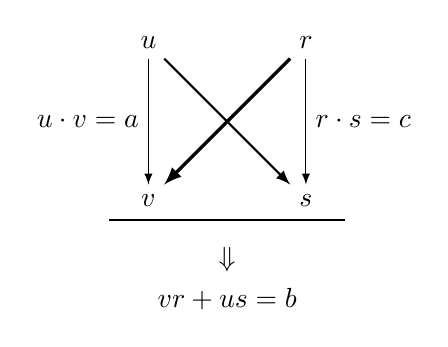
\begin{tikzpicture}[>=latex]
\node (A) at (0,0) {$u$};
\node (B) at (2,0) {$r$};
\node (C) at (0,-2) {$v$};
\node (D) at (2,-2) {$s$};    
\draw[->,thick] (A)--(D);
\draw[->,very thick] (B)--(C);
\draw [->] (A)--node[left]{$u\cdot v=a$}(C);
\draw [->] (B)--node[right]{$r\cdot s=c$}(D);
\draw (-.5,-2.25)--(2.5,-2.25);
\node at (1,-2.75){$\Downarrow$};
\node at (1,-3.25){$vr+us=b$};
\end{tikzpicture}    
\end{center}


要找这四个数$u,v,r,s$,可以这样去做:先找$a$的因数,使$u\cdot v=a$;再找$c$的因数,使$rs=c$;最后再试验$us+vr$是否等于$b$:
\begin{itemize}
    \item 如果$us+vr=b$,那么$ax^2+bx+c= (ux+r) (vx+s)$;
\item 如果$us+vr\ne b$,那么就要重新安排$u$、$v$、$r$、$s$的位置或按上法另找一组数,继续试验,直到符合要求为止.
\end{itemize}

\begin{example}
分解因式:
\[x^2-5x+6,\qquad x^2-x-12\]   
\end{example}

\begin{analyze}
    这两题中,$a=1$, 不难看出$u,v$只有都等于1的情形,因而我们只要能找出数$r,s$,满足$rs=c$, $r+s=b$, 即可将二次三项式$x^2+bx+c$分解为$(x+r)\cdot (x+s)$.
\end{analyze}

\begin{solution}
\begin{center}
    \begin{tikzpicture}
 \begin{scope}
\node (A) at (-.6,1.2) {$1$};
\node (B) at (.6,1.2) {$1$};
\node (C) at (-.6,0) {$1$};
\node (D) at (.6,0) {$6$};
\draw[very thick] (A)--(D);
\draw[very thick] (B)--(C);
\node at (0,-.5){$1+6=7$};
\node at (0,-1){(不合适)};
 \end{scope}   
 \begin{scope}[xshift=3cm]
    \node (A) at (-.6,1.2) {$1$};
    \node (B) at (.6,1.2) {$2$};
    \node (C) at (-.6,0) {$1$};
    \node (D) at (.6,0) {$3$};
    \draw[very thick] (A)--(D);
    \draw[very thick] (B)--(C);
    \node at (0,-.5){$2+3=5$};
    \node at (0,-1){(不合适)};
     \end{scope} 
     \begin{scope}[xshift=6cm]
        \node (A) at (-.6,1.2) {$1$};
        \node (B) at (.6,1.2) {$-2$};
        \node (C) at (-.6,0) {$1$};
        \node (D) at (.6,0) {$-3$};
        \draw[very thick] (A)--(D);
        \draw[very thick] (B)--(C);
        \node at (0,-.5){$-2+(-3)=-5$};
        \node at (0,-1){(合适)};
         \end{scope} 
\end{tikzpicture}
\end{center}
\[\therefore\quad x^2-5x+6=(x-2)(x-3)\]

\begin{center}
    \begin{tikzpicture}
 \begin{scope}
\node (A) at (-.6,1.2) {$1$};
\node (B) at (.6,1.2) {$-3$};
\node (C) at (-.6,0) {$1$};
\node (D) at (.6,0) {$4$};
\draw[very thick] (A)--(D);
\draw[very thick] (B)--(C);
\node at (0,-.5){$-3+4=1$};
\node at (0,-1){(不合适)};
 \end{scope}   
 \begin{scope}[xshift=5cm]
    \node (A) at (-.6,1.2) {$1$};
    \node (B) at (.6,1.2) {$3$};
    \node (C) at (-.6,0) {$1$};
    \node (D) at (.6,0) {$-4$};
    \draw[very thick] (A)--(D);
    \draw[very thick] (B)--(C);
    \node at (0,-.5){$3-4=-1$};
    \node at (0,-1){(合适)};
     \end{scope} 
\end{tikzpicture}
\end{center}
\[\therefore\quad x^2-x-12=(x+3)(x-4)\]

\end{solution}

\begin{example}
分解因式:
\[15x^2-7x-2,\qquad 11x^2-54x+63 \]
\end{example}


\begin{solution}
    \begin{center}
        \begin{tikzpicture}
     \begin{scope}
    \node (A) at (-.6,1.2) {$3$};
    \node (B) at (.6,1.2) {$1$};
    \node (C) at (-.6,0) {$5$};
    \node (D) at (.6,0) {$-2$};
    \draw[very thick] (A)--(D);
    \draw[very thick] (B)--(C);
    \node at (0,-.5){$5-6=-1$};
    \node at (0,-1){(不合适)};
     \end{scope}   
     \begin{scope}[xshift=5cm]
        \node (A) at (-.6,1.2) {$3$};
        \node (B) at (.6,1.2) {$-2$};
        \node (C) at (-.6,0) {$5$};
        \node (D) at (.6,0) {$1$};
        \draw[very thick] (A)--(D);
        \draw[very thick] (B)--(C);
        \node at (0,-.5){$-10+3=-7$};
        \node at (0,-1){(合适)};
         \end{scope} 
    \end{tikzpicture}
    \end{center}
    \[\therefore\quad 15x^2-7x-2=(3x-2)(5x+1)\]

    \begin{center}
        \begin{tikzpicture}
     \begin{scope}
    \node (A) at (-.6,1.2) {$11$};
    \node (B) at (.6,1.2) {$-63$};
    \node (C) at (-.6,0) {$1$};
    \node (D) at (.6,0) {$-1$};
    \draw[very thick] (A)--(D);
    \draw[very thick] (B)--(C);
    \node at (0,-.5){$-63-11=-74$};
    \node at (0,-1){(不合适)};
     \end{scope}   
     \begin{scope}[xshift=5cm]
        \node (A) at (-.6,1.2) {$11$};
        \node (B) at (.6,1.2) {$-21$};
        \node (C) at (-.6,0) {$1$};
        \node (D) at (.6,0) {$-3$};
        \draw[very thick] (A)--(D);
        \draw[very thick] (B)--(C);
        \node at (0,-.5){$-21-33=-54$};
        \node at (0,-1){(合适)};
         \end{scope} 
    \end{tikzpicture}
    \end{center}
    \[\therefore\quad 11x^2-54x+63=(11x-21)(x-3)\]
    
\end{solution}

\begin{example}
    分解因式:$6x^2-xy-12y^2$
\end{example}

\begin{analyze}
    遇到含有两个元的二次三项式,也可以与一元类似地作出因式分解.
    \begin{center}
        \begin{tikzpicture}
     \begin{scope}
    \node (A) at (-.6,1.2) {$2$};
    \node (B) at (.6,1.2) {$-4$};
    \node (C) at (-.6,0) {$3$};
    \node (D) at (.6,0) {$3$};
    \draw[very thick] (A)--(D);
    \draw[very thick] (B)--(C);
    \node at (0,-.5){$-12+6=-6$};
    \node at (0,-1){(不合适)};
     \end{scope}   
     \begin{scope}[xshift=3cm]
        \node (A) at (-.6,1.2) {$2$};
        \node (B) at (.6,1.2) {$3$};
        \node (C) at (-.6,0) {$3$};
        \node (D) at (.6,0) {$-4$};
        \draw[very thick] (A)--(D);
        \draw[very thick] (B)--(C);
        \node at (0,-.5){$9-8=1$};
        \node at (0,-1){(不合适)};
         \end{scope} 
         \begin{scope}[xshift=6cm]
            \node (A) at (-.6,1.2) {$2$};
            \node (B) at (.6,1.2) {$-3$};
            \node (C) at (-.6,0) {$3$};
            \node (D) at (.6,0) {$4$};
            \draw[very thick] (A)--(D);
            \draw[very thick] (B)--(C);
            \node at (0,-.5){$-9+8=-1$};
            \node at (0,-1){(合适)};
             \end{scope} 
    \end{tikzpicture}
    \end{center}
    \[\therefore\quad 6x^2-xy-12y^2=(2x-3y)(3x+4y)\]    
\end{analyze}

\begin{ex}
    用视察法分解因式:
\begin{multicols}{2}
    \begin{enumerate}
        \item $\poly{1,3,2}$
        \item $\poly{1,-1,-2}$
        \item $\poly{1,1,-30}$
        \item $\poly{1,-14,45}$
        \item $\poly{1,12,-64}$
        \item $\poly{3,-7,2}$
        \item $\polynomial[reciprocal, var=y]{4,1,-3}$
        \item $\polynomial[reciprocal, var=y]{10,-11,1}$
        \item $2ax+8x^2+3a^2$
        \item $14x^2+xy-3y^2$
        \item $\poly{1,0,-6,0,-27}$
        \item $a^6-7a^3-8$
    \end{enumerate}  
\end{multicols}

\end{ex}

综合以上各种分解因式的方法,一般可以按以下步骤考虑:
\begin{enumerate}
    \item 先考虑提取公因式法,
    \item 再考虑用公式或十字相乘法,
    \item 再考虑分组分解法.
\end{enumerate}

但是要注意:多项式的因式分解,和它的系数范围有密切关系,如:$x^2-2$在有理数范围内就认为不能再分解了,而在实数范围内,它又可以分解为:
\[x^2-2=(x+\sqrt{2})(x-\sqrt{2})\]
所以,在今后的分解因式时,如果没有特别指明,一般只要求在有理数范围内分解到不能再分解为止.

\begin{example}
    把$\poly{1,0,-3,0,2,0,0}$分解因式.
\end{example}

\begin{solution}
 \[\begin{split}
    \poly{1,0,-3,0,2,0,0}&=x^2\left(\poly{1,0,-3,0,2}\right)\\
    &=x^2(x^2-1)(x^2-2)\\
    &=x^2(x+1)(x-1)(x^2-2)    
 \end{split}\]   
\end{solution}


\begin{example}
    把$x^2+2xy+y^2-2x-2y-3$分解因式.
\end{example}

\begin{solution}
    \[\begin{split}
        x^2+2xy+y^2-2x-2y-3&=(x+y)^2 -2(x+y)-3\\
        &=(x+y-3)(x+y+1)    
    \end{split}\]
\end{solution}

\begin{example}
    把$\poly{1,1,1,1,0,0}$分解因式. 
\end{example}

\begin{solution}
    \[\begin{split}
        \poly{1,1,1,1,0,0}&=x^2\left(\poly{1,1,1,1}\right)\\
        &=x^2[x^2(x+1)+(x+1)]\\
        &=x^2(x+1)(x^2+1)       
    \end{split}\]
\end{solution}


\begin{ex}
 分解因式:
 \begin{enumerate}
     \item $a^2+2ab+b^2-ac-bc$
     \item $4m^2+4mn+n^2+6m+3n+2$
     \item $a^6-a^4+a^3-a$
     \item $\poly{1,-1,-2,2,-8,8}$
 \end{enumerate}   
\end{ex}

在运用乘法公式或分组分解因式时,有时需要将多项式作一些人为的变形,常见的是需要\textbf{添项}或\textbf{拆项}.

\begin{example}
    把$x^4+x^2y^2+y^4$分解因式.
\end{example}

\begin{solution}
\begin{align*}
    x^4+x^2y^2+y^4&=x^4+2x^2y^2+y^4 -x^2y^2 \tag{添项}\\
    &=(x^2+y^2)^2-(xy)^2\\
    &=(x^2+xy+y^2)(x^2-xy+y^2)
\end{align*}   
\end{solution}


\begin{example}
    把$a^4-11a^2+1$分解因式.
\end{example}

\begin{solution}
    \begin{align*}
        a^4-11a^2+1&=a^4-2a^2+1-9a^2 \tag{拆项}\\
        &=(a^2-1)^2-(3a)^2\\
        &=(a^2+3a-1)(a^2-3a-1)
    \end{align*}     
\end{solution}

\begin{ex}
    分解因式:
\begin{multicols}{2}
\begin{enumerate}
\item $\poly{1,0,-3,0,1}$
\item $\poly{1,0,0,0,4}$
\item $a^4-3a^2-18$
\item $x^4-27x^2y^2+y^4$
\end{enumerate}
\end{multicols}
\end{ex}

\subsection{待定系数法分解因式}
二元二次多项式
\[ax^2+bxy+cy^2+dx+ey+f\]
在一般情况下是不可约多项式.但在某些特殊情况下是能够分解成两个二元一次因式的.如何判断这样的多项式能否分解?如果能分解时,又怎样入手呢?我们将用待定系数法去解决这个问题.



\begin{example}
    把多项式$2x^2-3xy-2y^2+3x+4y-2$分解因式.
\end{example}

\begin{analyze}
   直接视察可知这个多项式的前三项是可
    分解的:$$2x^2-3xy-2y^2=(2x+y)(x-2y)$$
 因而我们推断:多项式$2x^2-3xy-2y^2+3x+4y-2$若能分解成两个一次式,则必然是$(2x+y+n)(x-2y+m)$的形式.我们只要能求出$m$、$n$,多项式即可分解因式;如果$m, n$不存在,就可断定,这个多项式不能分解因式.   
\end{analyze}

\begin{solution}
$\because\quad 2x^2-3xy-2y^2=(2x+y)(x-2y)$

$\therefore\quad $可设$2x^2-3xy-2y^2+3x+4y-2=(2x+y+n)(x-2y+m)$,即:
\[\begin{split}
   &\quad 2x^2-3xy-2y^2+3x+4y-2\\
   &=2x^2-3xy-2y^2+(2m+n)x+(m-2n)y+m\cdot n 
\end{split}\]

由多项式恒等,比较等式两边同类项的系数,可得:
\begin{align}
        2m+n=3\\
        m-2n=4\\
        m\cdot n=-2
\end{align}

由(5.1), (5.2)可解出$m=2$, $n=-1$.代入(1.3)满足.

$\therefore\quad 2x^2-3xy-2y^2+3x+4y-2=(2x+y-1) (x-2y+2)$
\end{solution}


\begin{example}
    将$x^2-y^2+2x+y-1$分解因式
\end{example}


\begin{solution}
    $\because\quad x^2-y^2=(x+y)(x-y)$

$\therefore\quad $可设$x^2-y^2+2x+y-1=(x+y+m) (x-y+n)$,即
\[x^2-y^2+2x+y-1=x^2-y^2+ (m+n) x+ (n-m) y+mn\]
    比较等式两边同类项的系数,得:    
\begin{align}
    m+n=2\\
    n-m=1\\
    m\cdot n=-1
\end{align}
由(5.4)、(5.5)可解出:$m=\frac{1}{2},\quad n=\frac{3}{2}$.但将$m,n$的值代入(5.6):
\[m\cdot n=\frac{1}{2}\cdot\frac{3}{2}\ne -1\]
即同时满足(5.4)、(5.5)、(5.6)的$m,n$不存在.

因此,$x^2-y^2+2x+y-1$是不可约多项式,不能再分解因式.
\end{solution}


\begin{example}
    已知$f(x)=\poly{1,0,4,3,k}$有一个因式$x^2+x+1$.试求$k$值及另外的因式.
\end{example}

\begin{solution}
    $\because\quad f(x)$为四次多项式,且有因式$x^2+x+1$.

    $\therefore\quad f(x)$的另一个因式必为二次式.

    不妨设$f(x)=(x^2+x+1)(ax^2+bx+c)$,即:
\[\begin{split}
    \poly{1,0,4,3,k}&=(x^2+x+1)(ax^2+bx+c)\\
    &=\poly{a,(a+b),(a+b+c),(b+c),c}
\end{split}\]
比较等式两边同类项的系数,得:
\[\begin{cases}
    a=1\\
    a+b=0\\
    a+b+c=4\\
    b+c=3\\
    c=k
\end{cases}\]
从中可解得:$a=1,\quad b=-1,\quad c=4,\quad k=4$.

因此,$f(x)=(x^2+x+1)(x^2-x+4)$,其中$x^2+x+1$与$x^2-x+4$都不可约.
\end{solution}

\begin{ex}
\begin{enumerate}
    \item 分解因式:
\begin{enumerate}
    \item $x^2+2xy-8y^2+2x+14y-3$;
    \item $x^2-8xy+15y^2+2x-4y-3$;
    \item $x^2+3xy+2y^2+4x+3y+1$.
\end{enumerate}
\item  已知$f(x)=\poly{3,-2,-32,66,a}$有一个因式是$\poly{1,2,-7}$.试求$a$的值及另外的因式.
\end{enumerate}    
\end{ex}

\section*{习题5.1}
\addcontentsline{toc}{subsection}{习题5.1}
\begin{enumerate}
    \item 填空:
\begin{enumerate}
    \item $-3a^3b^2c=abc(\qquad\qquad )$
    \item $mx^2+nx-p=m(\qquad \qquad)$
    \item $-12a^2b-3a^2b^2x+27ab^2=3ab(\qquad\qquad )$
    \item $3x^2y^3z^4-6x^3y^4z^2+18x^4y^2z^3=-3x^2y^2z^2(\qquad\qquad )$
\end{enumerate}
    \item 写出下列各题中的公因式:
\begin{enumerate}
    \item $5x^2y,\qquad 15xy^2,\qquad 45xyz$
    \item $24a^2(1-x)^2(x+y),\qquad 42ab(x-1)(x+y)^2$
    \item $-2(a+b)^2+4(a+b),\qquad (a+b)^2-3(a+b)^3$
    \item $(2x-4y)(2a-b),\qquad (x-y)(4a-2b)$
\end{enumerate}
    \item 用提取公因式法分解因式:
    \begin{enumerate}
        \item $-ax-ay+az$
        \item $14ab-35a^2-21a$
    \item $100m^2n-25mn^2+30m^2n^2$
    \item $a^m-a^{m+2}$
    \item $x(2a-3b)-y(3b-2a)$
    \item $a^2(x-y)^3+b^2(y-x)^3$
    \item $2a(x+y-z)+3b(y-z+x)-5c(z-x-y)$
    \item $5m^2n^2(a-b-c)-10m^2n^3(b+c-a)+75m^2n^4(b-a+c)$
\end{enumerate}
    \item 分组分解因式:
    \begin{multicols}{2}
    \begin{enumerate}
    \item $1-x-y+xy$
    \item $x^3-x+x^2-1$
    \item $ab-bc-b^2+ca$
    \item $ax+y-ay-x$
    \item $x^2+ax-y^2+ay$
    \item $x^3+x^2y-x^2z-xyz$
    \item $ax^2+bx^2-bx-ax+cx^2-cx$
    \item $x^3+9+3x^2+3x$
\end{enumerate}
\end{multicols}
    \item 将下列多项式展开后,再分解因式.
\begin{enumerate}
    \item $(ax-by)^2+(ay+bx)^2+c^2x^2+c^2y^2$
    \item $ab(c^2-d^2)-cd(a^2-b^2)$
\end{enumerate}
    \item 分解因式:
\begin{multicols}{2}
\begin{enumerate}
    \item $\poly{1,4,3}$
    \item $\poly{1,-11,10}$
    \item $\poly{1,-2,-48}$
    \item $2a^2+14ab+24b^2$
    \item $x^2+4xy-5y^2$
    \item $\poly{3,-7,2}$
    \item $\poly{6,-7,-3}$
    \item $3x^2 − 2xy − 8y^2$
    \item $(x^2-6)^2-25x^2$
    \item $\poly{1,-4.5,5}$
    \item $x^2 −7xy+10y^2$
    \item $\poly{1,2\frac{1}{2},1}$
    \item $\poly{1,3\frac{5}{12},2}$
    \item $\poly{20,-39,18}$
    \item $\poly{1,-5.6,6.4}$
    \item $2x^3 − 7x^2y + 3xy$
    \item $a^6+26a^3-27$
    \item $25x^{2n+2}-64x^{n+1}$
\end{enumerate}
\end{multicols}
    \item 在实数范围内分解因式:
    \begin{multicols}{2}
    \begin{enumerate}
        \item $\poly{3,2,-3}$
        \item $\poly{2,16,1}$
        \item $\poly{1,0,-5,0}$
        \item $a^4-27a^2+1$
\end{enumerate}
\end{multicols}
    \item 分解因式:
    \begin{multicols}{2}
        \begin{enumerate}
        \item $-x^2+12xy-36y^2$
    \item $25-20a+4a^2$
    \item $25x^4-10x^2y^2+y^4$
    \item $75-12x^2$
    \item $25t^2-0.09$
    \item $1-64a^2$
    \item $\poly{1,-\frac{2}{3},\frac{1}{9}}$
    \item $2mp^2-50m$
    \item $(x+1)^2-9(x-1)^2$
    \item $a^2-(2b+c)^2$
    \item $4(3p+5q)^2-9(2p-q)^2$
    \item $a^2x^{2n+1}-b^2x^{4n+2}$
    \item $8a^3+27b^3$
    \item $a-a^5$
    \item $(a+b)^3-8(2a-b)^3$
    \item $x^4+6x^2y^2+9y^4$
    \item $5x^6-10x^3y^3+5y^6$
    \item $18x^3y-36x^2y^2+18xy^3$
    \item $\poly{4,-8,4,0}$
    \item $a^2-b^2-c^2-2bc$
    \item $25-a^2+6ab-9b^2$
    \item $9x^2-4y^2-z^2+4yz$
    \item $a^2+2a+1-c^2+2cd-d^2$
    \item $a^6-64$
    \item $16x^3-\frac{1}{4}$
    \item $t^6-3t^4+3t^2-1$
\end{enumerate}
    \end{multicols}
    
    \item 用适当方法分解因式:
    \begin{multicols}{2}
\begin{enumerate}
    \item $16m^3+2n^3-2m-n$
    \item $a^4+2a^3b+8ab^3+16b^4$
    \item $x^3-64y^3+x^2-16y^2$
    \item $x^4-8x^2-9$
    \item $x^4-8x^2+\frac{1}{4}$
    \item $(x+y)^2-22x-22y+21$
    \item $a^2-2a(b-c)+(c-b)^2$
    \item $4x^2-12xy+9y^2-2x+3y-2$
    \item $x^6-3x^4+2x^2$
    \item $x^4+64y^4$
\end{enumerate}
\end{multicols}
    \item 先分解因式,再求值:
\begin{enumerate}
    \item $f(x,y)=xy-\frac{1}{2}(x^2+y^2)$,求:$f(75,65)$
    \item $\varphi(a,b)=6a^3b-3a^2b^2$,求:$\varphi\left(\frac{1}{2},\frac{2}{3}\right)$    
    \item $g(a,x,y)=x(a+3)-y(a+3)$,求:$g\left(4,\frac{3}{4},\frac{1}{2}\right)$
    \item $q(m,n)=m^2-n^2+(m+n)^2-m-n$.求:$q(1.5,-3.7)$
\end{enumerate}
    \item 证明:
\begin{enumerate}
    \item $47^6-47^5$能被46整除;
    \item $24^{10}+24^9$能被25整除;
    \item $5^{23}-5^{21}$能被24整除;
    \item $25^7+5^{13}$能被30整除;
    \item 对任意自然数$n$,$(n+8)^2-n^2$一定是8的倍数;
    \item $81^7-27^9-9^{13}$必定是45的倍数;
    \item 如果$m$及$n$都是正偶数,或都是正奇数时,那么$m^2-n^2$必定是4的倍数.
\end{enumerate}
    \item 用待定系数法分解因式:
    \begin{enumerate}
    \item $x^2+2xy+y^2+x+y-2$
    \item $x^2+xy-2y^2+2x+7y-3$
    \item $x^2+3xy+2y^2+4x+5y+3$
\end{enumerate}
    \item $m$是什么数值时,多项式$f(x)=mx^2-2xy-3y^2+3x-5y+2$能够分解为两个一次因式?并分解出来.
    \item 已知$g(x)=\poly{2,3,\ell,m}$有一个因式$\poly{1,1,-6}$,试求$\ell,m$的值,并把$g(x)$因式分解.
    \item 已知$f(x)=\poly{1,a,1,b,1}$有一个因式$\poly{1,-2,1}$,试求$a,b$的值,并把$f(x)$进行因式分解.
\end{enumerate}

\section{余式定理及其推论}
\subsection{余式定理}
运用综合除法,我们可以求得任一个多项式$f(x)$除以一次式$x-a$及$bx-a$的商式及余式.如果仔细观察每次做的结果,可以得出很重要而有趣的结论.我们还是先从例子谈起.

\begin{example}
已知$f(x)=x^3+3x^2-x-6$,

    试求:$f(x)$除以$x-2$及$f(x)$除以$x-a$的
    余式.

    再求:$f(2)$及$f(a)$的值.
\end{example}

\begin{solution}
用综合除法   
\begin{center}
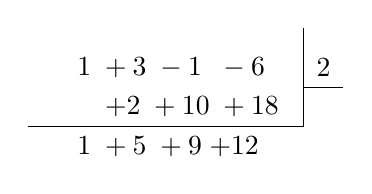
\begin{tikzpicture}
\node at (0,0.5) [right] {$1\; +3\; -1\;\; -6$};
\node at (0,0) [right] {$\quad  +2\; +10\; +18$};
\node at (0,-0.5) [right] {$1\;  +5\; +9\; \boxed{+12}$};
\draw (-.5,-.25)--(3,-.25)--(3,1);
\draw (3,.25)--(3.5,.25);
\node at (3.25,.5){$2$};

\end{tikzpicture}
\end{center}
$\therefore\quad f(x)$除以$x-2$,所得余式为一常数$12$.

\begin{center}
    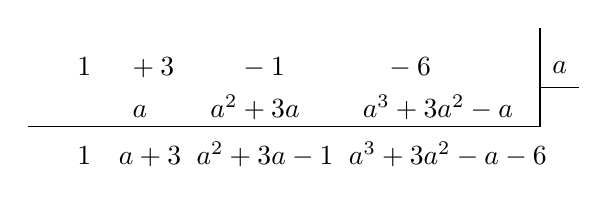
\begin{tikzpicture}
    \node at (0,0.5) [right] {$1\;\quad +3\;\qquad  -1\;\;\quad\quad\quad  -6$};
    \node at (0,0) [right] {$\qquad  a\; \quad \quad a^2+3a\;\quad\quad  a^3+3a^2-a$};
    \node at (0,-0.6) [right] {$1\quad  a+3\;\; a^2+3a-1\;\; \boxed{a^3+3a^2-a-6}$};
    \draw (-.5,-.25)--(6,-.25)--(6,1);
    \draw (6,.25)--(6.5,.25);
    \node at (6.25,.5){$a$};
    
    \end{tikzpicture}
    \end{center}
$\therefore\quad f(x)$除以$x-a$,所得余式为$a^3+3a^2-a-6$.
又:
\[\begin{split}
f(2)&= 2^3+3\x 2^2-2-6=12 \\
f(a)&= a^3+3a^2-a-6   
\end{split}\]
\end{solution}


由此看来,真是巧极了,$f(x)$除以$x-2$的余式正好等于$f(2)$,而$f(x)$除以$x-a$所得的余式,也恰好等于$f(a)$.我们不禁会问:

一般地多项式$f(x)=a_n x^n +a_{n-1}x^{n-1}+\cdots+a_1x+a_0$除以$x-a$时,所得的余式是否也等于$f(a)$呢?
以下定理可以做出肯定回答.

\begin{blk}{余式定理}
多项式$f(x)$除以$x-a$所得的余式等于$f(a)$.    
\end{blk}

\begin{proof}
    设多项式$f(x)$除以$x-a$所得的商式为
$q(x)$,余式为$r(x)$.由除法可得:
\[f (x) =q (x)\cdot  (x-a)+r(x)\]
但:$\because\quad r(x)$的次数低于$x-a$的次数,

$\therefore\quad r(x)$必为零或零次多项式,即$r(x)$必
    为一个常数$R$.

因而
\begin{equation}
    f (x) =q (x) \cdot  (x-a) +R
\end{equation}
这是一个恒等式,不论$x$取何值,总是成立的.今设$x=a$,等式(5.7)也应成立.

    于是就有:$f(a)=q(a)\cdot (a-a)+R$
因此: 
\begin{equation}
   R=f (a)  
\end{equation}
\end{proof}

    这就证明了余式定理.这个结论使我们在不做除法的前提下,也可以用求多项式的值来求出余式.


\begin{example}
  不做除法,求下列各题的余数:
  \begin{enumerate}
      \item $f(x)=x^3-2x+1$除以$x-\frac{1}{2}$.
      \item $\varphi(x)=\poly{1,2,0,4,1}$除以$x+2$.
  \end{enumerate}
\end{example}    
    


\begin{solution}
\begin{enumerate}
    \item $\because\quad f\left(\frac{1}{2}\right)=\frac{1}{8}-1+1=\frac{1}{8}$
    
    由余式定理
    \[\therefore\quad \text{余数}R=\frac{1}{8}\]

\item 同理,$\because\quad \varphi(-2)=16-16-8+1=-7$

\[\therefore\quad \text{余数}R=-7\]
\end{enumerate}

    
\end{solution}


\begin{example}
    求$f(x)=2x^3-3x^2+8x-14$除以$2x-3$的余数.
\end{example}

\begin{solution}
    由于$f(x)$除以$2x-3$所得余数与$f(x)$除
    以$x-\frac{3}{2}$所得的余数是相同的,所以
\[\begin{split}
f\left(\frac{3}{2}\right)&=2\x\left(\frac{3}{2}\right)^3-3\x\left(\frac{3}{2}\right)^2+8\x\frac{3}{2}-14\\
&=\frac{27}{4}-\frac{27}{4}+12-14=-2
\end{split}\]
可得:$f(x)$除以$2x-3$的余数为$-2$.
\end{solution}

\begin{example}
 求证$f(x)=x^4-1$可被$x-1$整除.   
\end{example}

\begin{analyze}
   要证明$f(x)$可被$x-1$整除,只要证明$f(x)$除以$x-1$所得余数是0即可.
\end{analyze}

\begin{proof}
\[\because\quad f(1)=1^4-1=0\]
\[\therefore\quad f(x)\text{除以}x-1\text{余数为0}\]
因此,$f(x)=x^4-1$能被$x-1$整除.
\end{proof}

\begin{example}
$f(x)=\poly{3,10,-15,-9,8,-7}$.求$f\left(-\frac{1}{3}\right)$的值.
\end{example}

\begin{note}
如果直接将$x=-\frac{1}{3}$代入$f(x)$求值,显
    然计算繁杂.若根据余式定理,由于$f\left(-\frac{1}{3}\right)$应等
    于$f(x)$除以$x+\frac{1}{3}$的余数,因而,可以用综合除法求
    出$f(x)$除以$x+\frac{1}{3}$的余数$R$.这要简便一些.
\end{note}

\begin{solution}
由综合除法
\begin{center}
    \begin{tikzpicture}
    \node at (0,0.5) [right] {$3\; +10\; -15\;\; -9\; +8\; -7$};
    \node at (0,0) [right] {$\quad  -1\quad -3\quad +6\; +1\; -3$};
    \node at (0,-0.6) [right] {$3\; +9\;\; -18\;\; -3\;\; +9\; \boxed{-10}$};
    \draw (-.5,-.25)--(5,-.25)--(5,1);
    \draw (5,.25)--(5.5,.25);
    \node at (5.25,.5){$-\tfrac{1}{3}$};
    
    \end{tikzpicture}
    \end{center}
可知:$f(x)$除以$x+\frac{1}{3}$的余数为$-10$,
\[\therefore\quad f\left(-\frac{1}{3}\right)=-10\]
\end{solution}

由余式定理,我们得到恒等式:
\begin{equation}
    f(x)=q(x)\cdot (x-a)+f(a)
\end{equation}

\begin{ex}
\begin{enumerate}
    \item 设$f(x)=\poly{1,-3,-5,20,-8}$,试分别求出$f(x)$除以下列各式的余数:
    \[x-1,\quad x+1,\quad x-2,\quad x+2,\quad 3x+1,\quad 3x-2 \]
    \item 用适当方法求值:
    \begin{enumerate}
        \item $f(x)=\poly{1,0,-12,0,15,-7}$,求$f(6)$.
        \item $\varphi(x)=\poly{1,0,-1,2}$,求$\varphi\left(-\frac{1}{2}\right)$.
    \end{enumerate}
    \item 证明:$\poly{1,1,-1,-2,-2,0}$能被$x-\sqrt{2}$整除.
\end{enumerate}
\end{ex}

\subsection{余式定理的推论}
由余式定理,可以得到以下四个重要推论:
\begin{blk}{推论1}
    如果$f(a)=0$,那么$(x-a)$必能整除$f(x)$;反过来,如果$x-a$能整除$f(x)$,那么$f(a)=0$.
\end{blk}

\begin{proof}
    如果$f(a)=0$,由等式(5.9)可得:
    \[f(x)=q(x) \cdot (x-a)\]    
    这就是说,余数$R=0$,$x-a$整除$f(x)$.
    
    反过来,如果$x-a$整除$f(x)$,即余数$R=0$,由余式定理$R=f(a)$.
    
$$\therefore\quad f (a) =0$$
\end{proof}

推论1的内容,也可以这样叙述:如果$f(a)=0$,那么,$f(x)$必定有因式$(x-a)$.反过来,也正确.因此,推论1也叫\textbf{因式定理}.可作为判断$x-a$是否是$f(x)$的因式的依据.

\begin{example}
    试证明:
\begin{enumerate}
    \item $x-2$是$f(x)=\poly{1,-5,12,-12}$的因式;
    \item $x-a$是$\varphi(x)=x^5-a^5$的因式.
\end{enumerate}
\end{example}

\begin{proof}
\begin{enumerate}
    \item $\because\quad f(2)=2^3-5\x 2^2+12\x2-12=0$
    
    $\therefore\quad $ 由推论1知道$x-2$是$f(x)$的因式.
    \item $\because\quad \varphi(a)=a^5-a^5=0$
    
    $\therefore\quad $ $x-a$是$x^5-a^5$的因式.
\end{enumerate}

\end{proof}

\begin{example}
试证明:对于正整数$n$,$x-y$是$x^n-y^n$的因式,而不是$x^n+y^n$的因式.
\end{example}

\begin{proof}
设$f(x)=x^n-y^n$,其中$y^n$\textbf{看作}常数项.

$\because\quad f (y) =y^n -y^n=0$

$\therefore\quad x-y$是$x^n-y^n$的因式.

又设$\varphi(x)=x^n+y^n$

$\because\quad \varphi(y) =y^n +y^n\ne 0$

$\therefore\quad x-y$不是$x^n+y^n$的因式.
\end{proof}

\begin{blk}{推论2}
如果多项式$f(x)$有两个不同的根$a$和$b$,那么,$(x-a)(x-b)$必能够整除$f(x)$,即$f(x)$必含有因式$(x-a)(x-b)$;反过来说,如果$f(x)$ 含有因式$(x-a)(x-b)$,也就是$f(x)$能够被$(x-a)(x-b)$整除,那么,$a$、$b$一定是$f(x)$的两个根.
\end{blk}

\begin{proof}
    由于$a$是$f(x)$的根,即:$f(a)=0$.
   
    $\because\quad $由推论1可知,$(x-a)$能整除$f(x)$.
    不妨设
    \begin{equation}
        f(x)=q_1(x)\cdot (x-a)
    \end{equation}
    将$x=b$代入恒等式(5.10),可得$f (b) =q_1 (b)\cdot (b-a)$

    $\because\quad b$也是$f(x)$的根
    
    $\therefore\quad f(b)=0$
    
    因而可以得到:$q_1(b)\cdot (b-a)=0$.
    
    但由于$b\ne a$,
    $\quad\therefore\quad b-a\ne 0$

    $\therefore\quad$由上式得出$q_1(b)=0$

    根据推论1,就说明$x-b$能够整除$q_1(x)$.
    
    再设
\begin{equation}
    q_1 (x) =q_2 (x) \cdot  (x-b)
\end{equation}
    
(5.11)式代入(5.10)式:
\[f (x) =q_2 (x) \cdot (x-b)\cdot (x-a)\]

这正说明$(x-a)(x-b)$可整除$f(x)$,也就是$f(x)$含有因式$(x-a)(x-b)$.

反过来,如果$f(x)=q(x)\cdot (x-a)·(x-b)$,不难由$f(x)=0$得出,$q(x)\cdot (x-a)(x-b)=0$,显然可以得出$f(x)$的两个根$x=a$, $x=b$.
    
    同理,我们可证明:如果$f(x)$有$k$个不同的根,$a_1,a_2,\cdots,a_k$,那
    么,$f(x)$能被$(x-a_1)(x-a_2)\cdots(x-a_k)$整除.即:
    \[f (x) =q (x) \cdot  (x-a_1) (x-a_2)\cdots (x-a_k)\] 
    
    反过来说,结论也是成立的.

\end{proof}

\begin{example}
证明:$f(x)=\poly{1,2,-4,-2,3}$能够被$x^2-1$整除.
\end{example}

\begin{proof}
由于$x^2-1=(x+1)(x-1)$,且:
\[\begin{split}
    f(-1)&=(-1)^4+2\x(-1)^3-4\x(-1)^2-2\x (-1)+3\\
&=1-2-4+2+3=0\\
f(1)&=1+2-4-2+3=0
\end{split}\]
$\therefore\quad x=-1,\; x=1$是$f(x)$的两个根.

因此,$f(x)$能被$(x+1)(x-1)=x^2-1$整除.

\end{proof}

\begin{example}
    $a$和$b$是什么值的时候,才能使多项式$f(x)=\poly{1,a,2,b,-2}$能被$\poly{1,-1,-2}$整除?
\end{example}

\begin{solution}
由于$x^2-x-2=(x-2)(x+1)$,且由题意必有:
\[\begin{split}
    f(2) &= 16+8a+8+2b-2=0\\
    f(-1)&=1-a+2-b-2=0
\end{split}\]
即:\[\begin{cases}
    4a+b=-11\\
    a+b=1
\end{cases}\]
解此方程组得:$a=-4,\quad b=5$.

所以,当$a=-4,\quad b=5$时,$f(x)$能被$x^2-x-2$整除.
\end{solution}

\begin{ex}
\begin{enumerate}
    \item 证明:$f(x)=x^3-4x^2+9$含有因式$x-3$.你能找出$f(x)$的另一个因式来吗?
    \item 已知$\pm 1$是$f(x)=\poly{2,3,-2,-3}$的两个根,试用除法求出$f(x)$的第三个根来.
    \item 证明$f(x)=\poly{1,-2,0,-1,-2}$能被$x^2-3x+2$整除.
    \item 如果$x-3$能整除$g(x)=x^3+ax^2-20x+6$,求$a$.
    \item 如果$(x+2)(x-4)$能整除$f(x)=2x^3-x^2+mx+n$.试求$m$及$n$的值.
\end{enumerate}
\end{ex}

\begin{blk}{推论3}
    一个$n$次多项式$f(x)$,至多只能有$n$个不同的根.
\end{blk}

\begin{proof}
假如一个$n$次多项式$f(x)$有$n+1$个不同的根$a_1,a_2,\ldots,a_n,a_{n+1}$,那么由推论2就知:
\[f (x) =q (x) \cdot  (x-a_1) (x-a_2)\cdots (x-a_n)(x-a_{n+1})\] 

这显然是不可能的.因为等式右边各因式的乘积的次数,肯定超过了$n$次,这和已知$f(x)$是$n$次多项式就矛盾了.

所以,$n$次多项式$f(x)$至多只能有$n$个不同的根.
\end{proof}

以上这种“说明一个结论的反面是不可能的,从而说明了结论的正确”的方法,称为反证法.

\begin{example}
    试证明多项式$ax^3+bx^2+cx+d\quad (a\ne 0)$至多只能有三个不同的根.
\end{example}


\begin{proof}
    假如这个三次多项式有4个不同的根$a_1,a_2,a_3,a_4$,那么,由余式定理的推论2可知:
\[ax^3+bx^2+cx+d=q (x) (x-a_1) (x-a_2) (x-a_3) (x-a_4)\]

这个等式的左边也是已知的3次多项式,但它的右边,显然至少是一个4次多项式,这是不可能的.

所以,这个三次多项式,不可能有4个或4个以上不同的根,至多只能有三个不同根.
\end{proof}


\begin{blk}{推论4}
    如果两个$n$次多项式$f(x),\; g(x)$在$x$取$a_1,a_2,a_3,\ldots,a_n,a_{n+1}$这$n+1$个不同的值时,
    它们所对应的值都相等,即
\[f (a_1) =g (a_1) ,\; \; f (a_2) =g (a_2) ,\;  \ldots,\;  f (a_{n+1}) =g (a_{n+1}) \]
那么,这两个多项式实是同一个多项式.即
\[f (x) =g (x) \]
\end{blk}

我们仍用反证法来证明这个推论.

\begin{proof}
假如这两个$n$次多项式不同,即$f(x)\ne g(x)$,那么,$f(x)-g(x)$就是一个次数不超过$n$的非零多项式.

又由已知,$f (a_1) =g (a_1) ,\; \; f (a_2) =g (a_2) ,\;  \ldots,\;  f (a_{n+1}) =g (a_{n+1})$,可以得出:$f (a_1) -g (a_1)=0 ,\; \; f (a_2) -g (a_2)=0 ,\;  \ldots,\;  f (a_{n+1}) -g (a_{n+1})=0$.这就是说,$a_1,a_2,\ldots,a_{n+1}$都是多项式$f(x)-g(x)$的根.这就是说:$f(x)-g(x)$的次数不超过$n$次,却有$n+1$个不同的根.这显然与推论3的结论是矛盾的.所以是不可能的.

因此,多项式$f(x)-g(x)$不可能是一个非零多项式,也就是说,$f(x)-g(x)$只能是一个零多项式了.即
\[f (x) -g (x) =0\]
因此,$f(x)=g(x)$.

\end{proof}

推论4告诉我们:只要给出在$x$取$n+1$个不同值时多项式相应的值,就可以唯一确定一个$n$次多项式.

\begin{example}
如果当$x$取$0, 1, 2$时,多项式分别取值$0,0,1$.试确定一个二次多项式$f(x)$.
\end{example}


\begin{solution}
$\because\quad f(0)=0,\quad f(1)=0$

$\therefore\quad f(x)$一定可被$x(x-1)$整除.

因而,可设$f(x)=kx(x-1)$.

又$\because\quad f(2)=1$,代入上式得
\[1=k\x2 (2-1) \]

$\therefore\quad k=\frac{1}{2}$.
因此,所求二次式为:
\[f(x)=\frac{1}{2}x(x-1)=\frac{1}{2}x^2-\frac{1}{2}x\]
\end{solution}

\begin{example}
试求一个三次多项式$g(x)$,使它满足
\[g (0) =g (1) =0,\quad g (2) =1,\quad g (3) =5\]
\end{example}

\begin{solution}
    $\because\quad g(0)=0,\quad g(1)=0$

$\therefore\quad g(x)$必含有因式$x(x-1)$

因而可设所求三次式为:
\begin{equation}
    g (x) =x (x-1) (Ax+B)
\end{equation}

又$\because\quad g(2)=1$ 及 $g(3)=5$,代入(5.12),得 
\[\begin{cases}
    1=2(2-1)(2A+B)\\
    5=3(3-1)(3A+B)
\end{cases}\Rightarrow\quad \begin{cases}
    4A+2B=1\\
    18A+6B=5
\end{cases}\]
由此解方程组,可得:$A=\frac{1}{3},\quad B=-\frac{1}{6}$.

因此,求得
\[g(x)=x(x-1)\left(\frac{1}{3}x-\frac{1}{6}\right)=\frac{1}{6}x(x-1)(2x-1)\]
\end{solution}

\begin{example}
已知$f(0)=5,\quad f(1)=5,\quad f(-1)=7,\quad f(2)=25,\quad f(-2)=17$.

试求:一个四次多项式$f (x)$.
\end{example}

\begin{note}
同以上两例一样,用待定系数法求出$f(x)$.但仔细观察所给条件,我们还可以更简便而巧妙地去解决.
\end{note}

\begin{solution}
    将所给条件可以变形为:  
\[\begin{split}
    f(0)-5&=0\\
    f(1)-5&=0\\
    f(-1)-5&=2\\
    f(2)-5&=20\\
    f(-2)-5&=12\\
\end{split}\]

因而,我们可以先求出另一个四次多项式$F(x)$,使$F(x)=f(x)-5$,当然就符合条件:
\[F(0)=0,\quad F (1) =0,\quad  F (-1) =2,\quad F (2) =20,\quad  F (-2) =12\]

这时,由推论2可设
$F (x) =x (x-1) (ax^2+bx+c)$.将条件$F(-1)=2,\quad F(2)=20,\quad F(-2)=12$分别代入上式,可得:
\[\begin{cases}
    F (-1) =2=-1 (-1-1) (a-b+c),\\
    F (2) =20=2 (2-1) (4a+2b+c),\\
    F (-2) =12=-2 (-2-1) (4a-2b+c). 
\end{cases}\]
即:\[\begin{cases}
    a-b+c=1\\
4a+2b+c=10\\
4a-2b+c=2
\end{cases}\]
解这个方程组,得:$a=1,\quad b=2,\quad c=2$.

因此,$F(x)=x(x-1)(x^2+2x+2)$,即:
\[F(x)=x^4+x^3-2x\]
所以,$f(x)-5=x^4+x^3-2x$,即:
\[f(x)=x^4+x^3-2x+5\]
\end{solution}

\begin{ex}
\begin{enumerate}
    \item 当$x$取$0,1,-\frac{3}{2}$时,$f(x)$的值分别为$-3,0,0$,试求一个二次多项式$f(x)$.
\item 若$f(0)=-2,\; f(-2)=0,\; f(1)=12$,试求二次三项式$f(x)$.
\item 当$y$取$0, 1, 2,-1$时,三次多项式$\varphi(y)$的值分别为$0, 0,-6,-12$,试求:$\varphi(y)$.
\item 已知$f(0)=15,\; f(1)=18,\; f(-1)=14$,试求$f(2)$及$f(-2)$的值.
\end{enumerate}
\end{ex}

\subsection{余式定理及其推论的应用}
对于整数系数多项式$f(x)$,还可以应用余式定理及其推论分解因式或求它的有理根.

先考察以下例子:
\[\begin{split}
    6x^2-7x+2&= (2x-1) (3x-2);\\
6x^3-35x^2+47x-12&= (2x-3) (3x-1)(x-4);\\
8x^4-24x^3-x+3&= (x-3) (2x-1)(4x^2+2x+1) .
\end{split}\]

由这几例中,不难看出:整系数多项式分解因式后,各因式的最高次项系数都是原多项式的最高次项系数的因数,且各因式的常数项也都是原多项式的常数项的因数.如:上面第一例中,$2, 3$都是6的因数;$-1,-2$都是2的因数.而在第二、三两例中,同样
有:$2, 3, 1$都是6的因数,$-3,-1,-4$都是$-12$的
因数及$1, 2, 4$是8的因数,$-3,-1,+1$是$+3$的因数.

一般地,对一元$n$次整系数多项式来说,同样因为
分解后的各因式最高次项(或常数项)的乘积应等于原多项式的最高次项(或常数项).所以,若$px+q$是整系数多项式$f(x)=a_nx^n+a_{n-1}x^{n-1}+\cdots +a_1x+a_0$的因式,那么,$p$一定是$a_n$的因数,$q$一定是$a_0$的因数.(这里$p$、$q$是互质的).

因此,当我们要对一整系数多项式进行因式分解时,就可以先将其可能含有的因式写出,再逐个用余式定理去检验,取真去伪,即可找出此多项式的各个因式.从而达到因式分解.


\begin{example}
    将$f(x)=\poly{1,-4,1,6}$分解因式.
\end{example}

\begin{analyze}
    如果$f(x)$有因式$px+q$,那么,$p$可能
取数$\pm1$;而$q$可能取数$\pm1,\;\pm2,\;\pm3,\;\pm6$.

若$p=1$,则因式$px+q$可能为:
\[x\pm1,\quad x\pm2,\quad x\pm3,\quad x\pm6\]

若$p=-1$,则因式$px+q$又可能为:
\[- (x\mp 1) ,\quad - (x\mp 2) ,\quad - (x\mp 3) ,\quad -(x\mp 6)\]

如果把只差一常数倍的因式,看作是相同的,那么,$f(x)$的所有因式可能是:
\[x-1,\quad x+1, \quad x-2,\quad x+2,\quad x-3,\quad x+3,\quad x-6,\quad x+6\]

根据余式定理推论1,我们可以由简单的因式开始,逐个进行判断.从而找出$f(x)$的所有因式来.    
\end{analyze}


\begin{solution}
$\because\quad f(1)\ne 0,\qquad \therefore\quad x-1$不是$f(x)$的因式.

$\because\quad f(-1)= 0,\qquad \therefore\quad x+1$是$f(x)$的因式.

同样,$\because\quad f(2)= 0,\qquad \therefore\quad x-2$是$f(x)$的因式.

$\because\quad f(3)= 0,\qquad \therefore\quad x-3$是$f(x)$的因式.

以下不必尝试,$f(x)$不会再有一次因式.因此:
\[\begin{split}
 f(x)&=\poly{3,-4,1,6}\\
 &=(x+1)(x-2)(x-3)   
\end{split}\]
\end{solution}

应当指出,象例5.38中,$f(x)$是一个三次式,在找到一个因式$x+1$后,可不必再去试了,只要用综合除法就可将$f(x)$分解了.
\begin{center}
\begin{tabular}{rrrr|r}
    1 &$-4$&1&6  &$-1$\\
    \cline{5-5}
    & $-1$ & 5& $-6$\\
    \cline{1-4}
    1&$-5$ & 6&0\\
\end{tabular}    
\end{center}
因此:
\[\begin{split}
    f(x)&=(x+1)(x^2-5x+6)\\
    &=(x+1)(x-2)(x-3)
\end{split}\]

\begin{example}
    将$f(x)=\poly{2,-1,-15,9,16,4}$ 分解因式.
\end{example}


\begin{solution}
$f(x)$的因式可能是:$x\pm 1,\quad x\pm 2,\quad x\pm 4,\quad 2x\pm 1$

$\because\quad f(1)=15\ne 0,\quad f(-1)=9\ne 0$

$\therefore\quad x\pm 1$不是$f(x)$的因式.

以下为方便起见,应用综合除法试验,这样一旦确定一个因式,也可写出另一个因式.
\begin{center}
    \begin{tabular}{rrrrrr|r}
       2   &  $-1$ &  $-15$  &  $+9$ & $+16$& $+4$  & 2\\
        \cline{7-7}
        & $+4$ & $+6$& $-18$& $-18$& $-4$\\
        \cline{1-6}
        2& $+3$ &$-9$ &$-9$&$-2$&  $\boxed{0}$\\
    \end{tabular}    
    \end{center}
因此:
\begin{equation}
    f(x)=(x-2)(\poly{2,3,-9,-9,-2})
\end{equation}

继续将$\poly{2,3,-9,-9,-2}$分解因式,它的因式还可能是:$x\pm 1,\quad x\pm 2,\quad 2x\pm 1$.
\begin{center}
    \begin{tabular}{rrrrr|r}
       2   &  $+3$ &  $-9$  &  $-9$ & $-2$  & 2\\
        \cline{6-6}
        & $+4$ & $+14$& $+10$& $+2$\\
        \cline{1-5}
        2& $+7$ &$+5$ &$+1$&  $\boxed{0}$\\
    \end{tabular}    
    \end{center}
    因此:
\begin{equation}
    \poly{2,3,-9,-9,-2}=(x-2)(\poly{2,7,5,1})  
\end{equation}

再将$\poly{2,7,5,1}$分解因式,它的因式可能是:$x\pm 1,\quad 2x\pm 1$.
\begin{center}
    \begin{tabular}{rrrr|r}
       2   &  $+7$ &  $+5$  &  $+1$  & $-\frac{1}{2}$\\
        \cline{5-5}
        & $-1$ & $-3$& $-1$\\
        \cline{1-4}
        2& $+6$ &$+2$&  $\boxed{0}$\\
    \end{tabular}    
    \end{center}
    因此:$\poly{2,7,5,1}=\left(x+\frac{1}{2}\right)(\poly{2,6,2})$,即
\begin{equation}
    \poly{2,7,5,1}=\left(2x+1\right)(\poly{1,3,1})
\end{equation}

在有理数范围内,$\poly{1,3,1}$已不能再分解.

综合(5.13)、(5.14)、(5.15)可得:
\[f(x)=(x-2)(x-2)(2x+1)(\poly{1,3,1})\]

\end{solution}

\begin{example}
把$f(x)=\poly{6,5,3,-3,-2}$分解因式.
\end{example}

\begin{solution}
因式$px+q$可能是:$x\pm 1,\quad x\pm 2,\quad 2x\pm 1,\quad 3x\pm 1,\quad 3x\pm 2,\quad 6x\pm 1$

逐个试除,可得:
\begin{center}
    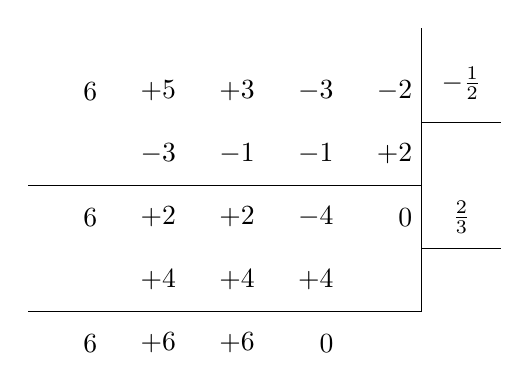
\begin{tikzpicture}
\foreach \x/\xtext in {0/6,1/+6,2/+6,3/\boxed{0}}
{
    \node at  (\x,0)[left]{$\xtext$};
}        
\foreach \x/\xtext in {1/+4,2/+4,3/+4}
{
    \node at  (\x,.8)[left]{$\xtext$};
}  
\foreach \x/\xtext in {0/6,1/+2,2/+2,3/-4, 4/\boxed{0}}
{
    \node at  (\x,1.6)[left]{$\xtext$};
}  
\foreach \x/\xtext in {1/-3,2/-1,3/-1, 4/+2}
{
    \node at  (\x,2.4)[left]{$\xtext$};
}  
\foreach \x/\xtext in {0/6,1/+5,2/+3,3/-3, 4/-2}
{
    \node at  (\x,3.2)[left]{$\xtext$};
}  
\draw (-1,.4)--(4,.4);  \draw (-1,2)--(4,2);\draw(4,.4)--(4,4);
\node at (4.5,3.3){$-\frac{1}{2}$};
\node at (4.5,1.6){$\frac{2}{3}$};
\draw (4,1.2)--(5,1.2); \draw (4,2.8)--(5,2.8);
 \end{tikzpicture}    
\end{center}

因此:$f(x)=\left(x+\frac{1}{2}\right)\left(x-\frac{2}{3}\right)(\poly{6,6,6})$
即:
\[f(x)=(2x+1)(3x-2)(\poly{1,1,1})\]
在我们进行因式分解时,不难看出,若$f(x)$含有因式$px+q$,则一定有$f\left(-\frac{q}{p}\right)=0$,因而,$x=-\frac{q}{p}$必然是$f(x)$的有理数根,如:
\[f(x)=(2x+1)(3x-2)(\poly{1,1,1})\]
$\therefore\quad f(x)$的有理根就是:$x_1=-\frac{1}{2},\quad x_2=\frac{2}{3}$.
\end{solution}


\begin{example}
    求方程$2x^4+x^3+12=17x^2+16x$的有理数根.
\end{example}

\begin{solution}
原方程变形为:$\poly{2,1,-17,-16,12}=0$

方程左边的多项式,可能有因式:$x\pm 1,\quad x\pm 2,\quad x\pm 3,\quad x\pm 4,\quad x\pm 6,\quad 2x\pm 1,\quad 2x\pm 3$
因而,此方程的有理根可能是:
\[x=\pm 1,\quad x=\pm 2,\quad x=\pm 3,\quad x=\pm 4,\quad x=\pm 6,\quad x=\pm \frac{1}{2},\quad x=\pm \frac{3}{2} \]
逐个去进行试除,即可找到方程的根.
\begin{center}
    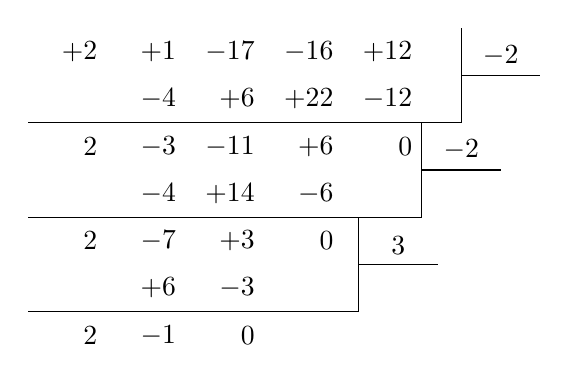
\begin{tikzpicture}[yscale=.6]
\foreach \x/\xtext in {0/2,1/-1,2/\boxed{0}}
{
    \node at  (\x,0)[left]{$\xtext$};
}        
\foreach \x/\xtext in {1/+6,2/-3}
{
    \node at  (\x,1)[left]{$\xtext$};
}  
\foreach \x/\xtext in {0/2,1/-7,2/+3,3/\boxed{0}}
{
    \node at  (\x,2)[left]{$\xtext$};
}  
\foreach \x/\xtext in {1/-4,2/+14,3/-6}
{
    \node at  (\x,3)[left]{$\xtext$};
}  
\foreach \x/\xtext in {0/2,1/-3,2/-11,3/+6, 4/\boxed{0}}
{
    \node at  (\x,4)[left]{$\xtext$};
}  
\foreach \x/\xtext in {1/-4,2/+6,3/+22, 4/-12}
{
    \node at  (\x,5)[left]{$\xtext$};
} 
\foreach \x/\xtext in {0/+2,1/+1,2/-17,3/-16, 4/+12}
{
    \node at  (\x,6)[left]{$\xtext$};
} 
\draw (-1,.5)--(3.2,.5)--(3.2,2.5)--(4,2.5)--(4,4.5)--(4.5,4.5)--(4.5,6.5);
\draw (-1,2.5)--(3.2,2.5);
\draw (-1,4.5)--(4,4.5);
\draw (3.2,1.5)--node[above]{3}(4.2,1.5);
\draw (4,3.5)--node[above]{$-2$}(5,3.5);
\draw (4.5,5.5)--node[above]{$-2$}(5.5,5.5);
 \end{tikzpicture}    
\end{center}
因此:$(x+2)(x+2)(x-3)(2x-1)=0$,
原方程的有理根是:
\[x_1=x_2=-2,\qquad x_3=3,\qquad x_4=\frac{1}{2}\]
\end{solution}

\begin{ex}
\begin{enumerate}
    \item 分解因式:
\begin{enumerate}
    \item $\poly{1,0,-7,6}$
    \item $\poly{1,6,11,6}$
    \item $\poly{1,0,-2,3,-2}$
    \item $\poly{1,-10,35,-50,24}$
    \item $\poly{2,-1,-9,13,-5}$
    \item $\poly{3,-3,-13,-11,-10,-6}$
\end{enumerate}
    \item 求下列多项式或方程的有理根.
\begin{enumerate}
    \item $\poly{1,-5,-2,24}=0$
    \item $\poly{2,-5,3,4,-6}$
    \item $\poly{12,-20,-11,5,2}=0$
    \item $\poly{16,0,-24,16,-3}$
\end{enumerate}
\end{enumerate}
\end{ex}


\subsection{根与系数的关系}
在本章第一节因式分解中,我们已经知道:当$b^2-4ac\ge 0$时,二次三项式$ax^2+bx+c\quad (a\ne 0)$利用配方法可以分解为 $ax^2+bx+c=a(x-x_1)(x-x_2)$的形式.其中
\[x_1=\frac{-b+\sqrt{b^2-4ac}}{2a},\qquad x_2=\frac{-b-\sqrt{b^2-4ac}}{2a}\]
正好是这个二次三项式的两个实根.

由此,我们进一步可以探讨“根与系数”之间存在的内在关系:
\[\begin{split}
    ax^2+bx+c&=a (x-x_1) (x-x_2)\\
&=ax^2-a(x_1+x_2)x+ax_1\cdot x_2
\end{split}\]

比较上边等式两边同类项的系数,得
\[b=-a(x_1+x_2),\qquad c=ax_1\cdot x_2 \]
\[\therefore\quad x_1+x_2=-\frac{b}{a},\qquad x_1\cdot x_2=\frac{c}{a}\]

这就是说:
\begin{blk}{}
    二次三项式$ax^2+bx+c\quad (a\ne 0)$(或一元二次方
程$ax^2+bx+c=0\quad (a\ne 0)$ ),如果有两个实根$x_1$、$x_2$,那么,这两个根与系数间一定有关系式:
\[ x_1+x_2=-\frac{b}{a},\qquad x_1\cdot x_2=\frac{c}{a} \]
\end{blk}

这就启发我们去考虑:一元$n$次多项式
$a_nx^n+a_{n-1}x^{n-1}+a_{n-2}x^{n-2}+\cdots+a_1x+a_0\quad (a_n\ne 0)$
的根与系数之间有什么关系呢?不妨以一元三次多项式(或方程)为例,我们作以下分析:

设三次多项式$\poly{a,b,c,d}\quad (a\ne 0)$有三个根$x_1,x_2,x_3$.由余式定理推论2可知:
\[ \poly{a,b,c,d}=a(x-x_1)(x-x_2)(x-x_3) \]
即:
\[\begin{split}
    \poly{a,b,c,d} &= ax^3-a(x_1+x_2+x_3)x^2\\
    &\qquad +a(x_1x_2+x_1x_3+x_2x_3)x-ax_1x_2x_3
\end{split}\]

比较等式两边同类项的系数,得:
\[\begin{split}
    a&=a\\
    b&=-a(x_1+x_2+x_3)\\
    c&=a(x_1x_2+x_1x_3+x_2x_3)\\
    d&=-ax_1\cdot x_2\cdot x_3
\end{split}\]

因此,可得出根与系数的关系如下:
\[ \begin{cases}
    x_1+x_2+x_3 =-\frac{b}{a}\\
    x_1x_2+x_1x_3+x_2x_3=+\frac{c}{a}\\
    x_1\cdot x_2\cdot x_3=-\frac{d}{a}
\end{cases} \]

这就是说,一元三次多项式的三个根之和等于二次项系数除以首项系数的相反数;三个根两两乘积的
和等于一次项系数除以首项系数;三个根之积等于常数项除以首项系数的相反数.

以上这种关系,可以类似地推广到一元$n$次多项式的情形.这就是韦达定理的内容.

\begin{blk}{韦达定理}
设一元$n$次多项式$$f(x)=a_nx^n+a_{n-1}x^{n-1}+a_{n-2}x^{n-2}+\cdots+a_1x+a_0\quad (a_n\ne 0)$$
有$n$个根$x_1,x_2,\ldots,x_n$.那么,这$n$个根与系数之间有以下关系:
\begin{itemize}
    \item $n$个根之和$(x_1+x_2+\cdots+x_n)$等于$x^{n-1}$的系数除以首项系数的相反数,即:$
    -\frac{a_{n-1}}{a_n}$;
    \item $n$个根的所有两两乘积之和$(x_1x_2+\cdots+x_{n-1}x_n)$等于$x^{n-2}$的系数除以首项系数,即:$
    \frac{a_{n-2}}{a_n}$;
    \item $n$个根的所有三个根乘积之和$(x_1x_2x_3+\cdots+x_{n-2}x_{n-1}x_n)$等于$x^{n-3}$的系数除以首项系数的相反数,即:$-\frac{a_{n-3}}{a_n}$;
    \item …………
    \item $n$个根的所有$(n-1)$个根乘积之和$(x_1x_2\cdots x_{n-1} +\cdots+ x_2x_3\cdots x_n)$等于$x$的系数除以首项系数再乘以$(-1)^{n-1}$,即:$ (-1)^{n-1}\frac{a_{1}}{a_n}$;
    \item $n$个根的乘积$x_1x_2\cdots x_n$就等于常数项除以首项系数再乘以$(-1)^{n}$,即:$ (-1)^{n}\frac{a_{0}}{a_n}$.
\end{itemize}
\end{blk}

如果应用韦达定理,我们就可以把一元二次方程$ax^2+bx+c=0\quad (a\ne 0)$即 $x^2+\frac{b}{a}x+\frac{c}{a}=0$写成以下形式:
\[x^2- (x_1+x_2) x+x_1\cdot x_2=0\]
其中,$x_1$、$x_2$是一元二次方程的两个根.

同样,一元三次方程,也可以写成:
\[x^3- (x_1+x_2+x_3) x+ (x_1x_2+x_1x_3+x_2x_3) x
-x_1\cdot x_2\cdot x_3=0\]

这样一来,如果已知方程的根,就可以反求出这个方程.

\begin{example}
    如果一个三次方程的根是1, 2, 3,试求这个三次方程.
\end{example}

\begin{solution}
由于:\[\begin{split}
    x_1+x_2+x_3 &=1+2+3=6\\
    x_1x_2+x_1x_3+x_2x_3&=2+3+6=11\\
    x_1x_2x_3&=6
\end{split}\]

由韦达定理可知所求三次方程为:
\[\poly{1,-6,11,-6}=0\]
\end{solution}

\begin{example}
    如果方程$\poly{1,-12,44,k}=0$的三个根为:$a-d,\; a,\; a+d$.试求这个方程的根及$k$值.
\end{example}

\begin{solution}
    由韦达定理可知:
\begin{align}
(a-d)+a+(a+d)&=12\\
a(a-d)+(a-d)(a+d)+a(a+d)&=44\\
(a-d)\cdot a\cdot (a+d)&=-k
\end{align}
解(5.16)可得:$a=4$;代入(5.17)又可解出:$d=\pm 2$.

$\therefore\quad $方程的三个根为:$2,\quad 4,\quad 6$

由(5.18)可求出:$k=-48$.
\end{solution}

\begin{example}
试作一个一元二次方程,使它的根正好是方程$x^2-x-6=0$的二根的倒数.
\end{example}


\begin{solution}
设$x^2-x-6=0$的两根为$\alpha,\beta$.则由题意,所求一元二次方程的根就应该是$\frac{1}{\alpha},\frac{1}{\beta}$.

又由韦达定理知:$\alpha+\beta=1,\quad \alpha\beta=-6$,因此:
\[\begin{split}
    \frac{1}{\alpha}+\frac{1}{\beta}&=\frac{\alpha+\beta}{\alpha\beta}=-\frac{1}{6}\\
    \frac{1}{\alpha}\cdot \frac{1}{\beta}&=\frac{1}{\alpha\beta}=-\frac{1}{6}\\
\end{split}\]
所以,所求的方程是:$x^2+\frac{1}{6}x-\frac{1}{6}=0$,即:
\[ 6x^2+x-1=0 \]
\end{solution}


\begin{ex}
\begin{enumerate}
    \item 已知方程的根,求作方程:
    \begin{enumerate}
        \item $-2,\quad  5$;
        \item $-1,\quad 0,\quad 1$;
        \item $2,\quad 3,\quad 4,\quad 5$.
    \end{enumerate}
    \item 试作一个一元二次方程.使它的二根分别是方程$x^2-12x+32=0$的二根的平方.
\end{enumerate}
\end{ex}

\begin{example}
    不解方程,试求方程$2x^2-x-15=0$的根的平方和与立方和.
\end{example}


\begin{solution}
    设$2x^2-x-15=0$的二根为$x_1,x_2$,
    则由韦达定理知:$x_1+x_2=\frac{1}{2},\qquad x_1x_2=-\frac{15}{2}$.

    因此:
\[\begin{split}
   x^2_1+x^2_2&=(x_1+x_2)^2-2x_1x_2\\ 
    &=\frac{1}{4}-2\x\left(-\frac{15}{2}\right)
    =15\frac{1}{4}\\
x^3_1+x^3_2&=(x_1+x_2)^3-3x_1x_2(x_1+x_2)\\
&=\frac{1}{8}-3\x\left(-\frac{15}{2}\right)\x\frac{1}{2}\\
&=\frac{1}{8}+\frac{45}{4}=\frac{91}{8}=11\frac{3}{8}    
\end{split}\]

\end{solution}


\begin{example}
不解方程,试求$\poly{1,1,2,1,1}=0$的根的平方和.
\end{example}

\begin{solution}
 设$\poly{1,1,2,1,1}=0$的四个根是$x_1,x_2,x_3,x_4$.则由韦达定理得:
\[\begin{cases}
  x_1+x_2+x_3+x_4=-1\\
  x_1x_2+x_1x_3+x_1x_4+x_2x_3+x_2x_4+x_3x_4=2\\
  x_1x_2x_3+x_1x_2x_4+x_2x_3x_4+x_1x_3x_4=-1\\
  x_1x_2x_3x_4=1  
\end{cases}\]
因此:
\[\begin{split}
  &\quad  x^2_1+x_2^2+x_3^2+x_4^2\\
&=(x_1+x_2+x_3+x_4)^2-2(x_1x_2+x_1x_3+x_1x_4+x_2x_3+x_2x_4+x_3x_4)\\
&=(-1)^2-2\x 2=-3
\end{split}\]
\end{solution}

\begin{example}
如果方程$x^2+3x+m=0$的两根差是5,求$m$值及两根.
\end{example}

\begin{solution}
    设两根为$x_1,x_2$,由韦达定理及题意,得
\[\begin{cases}
    x_1+x_2=-3\\
    x_1-x_2=5
\end{cases}\]
解方程组可得:$x_1=1,\quad x_2=-4$

因此:$m=x_1\cdot x_2=-4$.
\end{solution}

\begin{ex}
\begin{enumerate}
    \item 已知方程$x^2-4x-12=0$的一根为$-2$,求另一根.
    \item 不解方程,求出$3x^2-4x-15=0$的两根的平方和及平方差.
    \item 方程$x^2+px+45=0$的两根差的平方是144,求$p$值.
\end{enumerate}
\end{ex}

\section*{习题5.2}
\addcontentsline{toc}{subsection}{习题5.2}

\begin{enumerate}
    \item 用余式定理求下列各题的余数:
\begin{enumerate}
    \item $f(x)=\poly{3,-2,5,-4,3}$ 除以 $x-1$
    \item $f(x)=\poly{2,3,-5,1}$ 除以 $x+2$
    \item $g(x)=\poly{9,-3,6,-15}$ 除以 $x+\frac{1}{3}$
    \item $g(x)=\poly{1,0,0,1,-1}$ 除以 $2x-1$
    \item $\varphi(x)=\poly{1,-1,2,1,-1,-2}$ 除以 $5x+3$
\end{enumerate}    
    
\item 用综合除法求值:
\begin{enumerate}
    \item $f(x)=\poly{2,7,-14,6,7}$.求:$f(-5)$.
    \item $g(x)=\poly{6,8,-5,7,-3}$.求:$g\left(\frac{2}{3}\right)$的值.
\end{enumerate}

\item 不作除法,证明:
\begin{enumerate}
    \item $(x-1)^3-2(x-1)^2+3(x-1)-6$能被$x-3$整除.
    \item $a^3+a^2b-3ab^2+b^3$能被$a-b$整除.
\end{enumerate}

\item 证明:若$n$是奇数时,$x+y$是$x^n+y^n$的因式;若$n$是偶数时,$x+y$不是$x^n+y^n$的因式.

\item 证明:$\poly{1,-2,-4,3,-3,11,-6}$能被$\poly{1,-1,-6}$整除.

\item 证明:$f(x)=\poly{1,-4,1,6}$必有因式$(x-2)(x+1)$.
\item 如果$\poly{1,3,4,a,11}$能被$x+1$整除,试求$a$的值.
\item 当$a$为何值时:
\begin{enumerate}
    \item $f(x)=\poly{2,0,-3,11,-1,a}$除以$x+2$能余3?
    \item $g(x)=\poly{1,-3,5,a}$除以$x-1$能余4?
    \item $\varphi(x)=\poly{2,-3,a,-6}$除以$2x-4$能余6?
\end{enumerate}

\item 若用$x+1$及$x-1$去除多项式$\poly{2,-3,-a,-b}$分别余7及5.试求$a,b$的值.

\item 已知:$f(x)=\poly{1,-6,m,n}$能被$x^2-4x+3$
整除,试求$f\left(\frac{1}{2}\right)$及$f\left(-\frac{1}{2}\right)$.

\item 如果$g(x)=ax^2+bx+c$能被$x+1$整除,而且被$x-2$与$x+2$除时分别余2与$-3$,试求这个多项式$g(x)$.

\item 如果一个二次三项式$g(x)$的两根为1和2,且$g(3)=4$,试求出这个三项式$g(x)$.

\item 求一个一元三次多项式$f(x)$,使$f(1)=f(-1)=f(2)=0$,且$f(-2)=-12$.
\item 当$x$取$-1, 0, 2$时,二次三项式$\varphi(x)$分别取值$-6,1,-3$.试求此三项式$\varphi(x)$.
\item 如果$f(0)=10$, $f(1)=14$, $f(-1)=10$, 以及$f(-2)=8$,试求一个三次多项式$f(x)$.

\item 求下列整系数方程的有理根.
\begin{multicols}{2}
    \begin{enumerate}
    \item $\poly{1,-4,1,6}=0$
    \item $\poly{1,-8,13,-6}=0$
    \item $\poly{9,0,-13,6}=0$
    \item $\poly{1,-7,5,7,-6}=0$
    \item $\poly{1,5,8,1,-15}=0$
    \item $\poly{1,2,2,4,5,2}=0$
\end{enumerate}
\end{multicols}

\item 若方程$(a-b)x^2+(b-c)x+(c-a)=0$有一个根是1,
试求它的另一根.
\item 若方程$x^2+3x+m=0$的一根是另一根的2倍,求$m$的值.
\item 方程$x^3-px^2+11x-6=0$ 的三个根的平方和等于14.试求$p$的值.
\item 求作一个方程,使它的根是:
\begin{multicols}{2}
    \begin{enumerate}
    \item $\frac{3}{4}$ 和 $\frac{4}{3}$
    \item $\frac{1}{5}$ 和 $-\frac{1}{5}$ 和 $1$
\end{enumerate}
\end{multicols}

\item 求作一个三次方程,使它的根分别是方程$x^3+px^2+qx+r=0$的根的倒数.

\item 如果设$\alpha,\beta,
\gamma$是$\poly{1,1,-2,3}=0$的根,试作出根是
$y_1=\beta\gamma$, $y_2=\alpha\gamma$, $y_3=\alpha\beta$的新的三次方程.

\item 已知$2x^3-6x+8=0$的三根是$\alpha,\beta,
\gamma$.试求以下各式的值:
\begin{multicols}{2}
    \begin{enumerate}
    \item $(\alpha+\beta+\gamma)^2$ 
    \item $\alpha^2+\beta^2+\gamma^2$ 
    \item $\frac{1}{\alpha}+\frac{1}{\beta}+\frac{1}{\gamma}$
    \item $\beta^2\gamma^2+\alpha^2\gamma^2+\alpha^2\beta^2$
\end{enumerate}
\end{multicols}

\item 证明$f(x)=2x^2+8x+9$除以$(x-m)$,所得的余数都是正数.

\item 如果$f(a)=1$,试求$x^2\cdot f(x)$除以$x-a$所得的余数.

\item $f(2)=2$、$f(-3)=4$, 求$f(x)$除以$x^2+x-6$的余式.

\end{enumerate}


\section{辗转相除法}
\subsection{公因式与最高公因式}
在小学算术中,我们已经知道:如果一个整数$c$,同时是整数$a$和$b$的约数,那么,$c$就叫做$a$、$b$的公约数(公因数).例如:3就是12和18的公约数.当然,两个整数的公约数还可以有许多,如:$\pm 1,\pm 2,\pm 3,\pm 6$都是12和18的公约数(公因数).

两个数$a$、$b$的公约数中,最大的一个$d$,叫做这两个数的最大公约数.记作$(a,b)=d$.例如:$(12, 18)=6$.

如果两个数$a$、$b$的最大公约数$(a,b)=1$,那么,我们称$a$、$b$是两个互质的数,例如:
\[\because\quad (3,5)=1,\qquad \therefore\quad \text{3与5是互质的}\]

要求两个数的最大公约数,只要将它们分解为质因数,选出它们所有的公约数的最低次方连乘即可.

例如,求$(168,756)$
\begin{center}
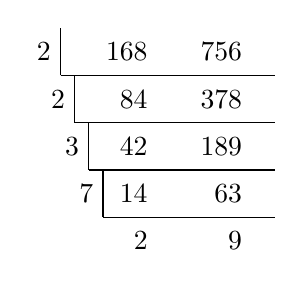
\begin{tikzpicture}[scale=.6]
\foreach \y/\ytext in {0/2, 1/14,2/42,3/84,4/168}
{
    \node at (0, \y)[left]{\ytext};
}
\foreach \y/\ytext in {0/9, 1/63,2/189,3/378,4/756}
{
    \node at (2, \y)[left]{\ytext};
}
\foreach \y/\x in {.5/7,1.5/3,2.5/2,3.5/2}
{
    \draw (-1-\y*0.3,\y)--(2.5,\y);
    \draw (-1-\y*.3,\y)--node[left]{\x}(-1-\y*.3,\y+1);
}

\end{tikzpicture}
\end{center}
\[\therefore \quad (168, 756)=2\x 2\x 3\x 7=84\]

对于多项式,我们有类似的概念:如果一个多项式$h(x)$,同时是两个多项式$f(x)$和$g(x)$的因式,那么,$h(x)$就叫做$f(x)$与$g(x)$的\textbf{公因式}.例如:$x-1$就是$x^2-1$和$x^3-1$的公因式.两个多项式的公因式可以有许多,如$x-1$, $x+1$, $x^2-1$都是$x^2-1$, $x^4+x^3-x-1$的公因式.特别注意,任何一个非零数(即零次多项式),都是$x^2-1$, $x^4+x^3-x-1$的公因式.

在两个多项式$f(x)$与$g(x)$的所有公因式中,次数最高的公因式$d(x)$,就叫做这两个多项式的\textbf{最高公因式},记作:$(f(x),g(x))=d(x)$.

例如:$f(x)=6x^4-6x^2=6x^2(x+1)(x-1)$, 
$g (x) =3x^2-3=3 (x+1) (x-1)$

因而可知:$1$, $3$, 任一非零数$a$, $x+1$, $x-1$, $2x+2$, …… 以及$x^2-1=(x+1)(x-1)$, $5x^2-5=5(x+1)(x-1)$, …… 都是$f(x)$与$g(x)$的公因式.这里也可以看出:公因式中,次数最高的也不只一个:$x^2-1$,$5x^2-5$, $\frac{1}{3}x^2-\frac{1}{3}$等都是$f(x),g(x)$的最高公因式.

但注意:这些最高公因式之间,只是相差一个常数倍(零次多项式),因此,我们约定:\textbf{在求两个多项式的最高公因式时,零次公因式(常数)不必考虑,只要各非零次项系数化为最简即可}.如在上例中,
\[(f(x),g(x))=(x+1)(x-1)=x^2-1\]
\begin{example}
求$\varphi(x)=\poly{4,4,1}$与$R(x)=\poly{8,12,6,1}$的最高公因式.
\end{example}

\begin{solution}
由于:\[\begin{split}
    \varphi(x)&=\poly{4,4,1}=(2x+1)^2\\
    R(x)&=\poly{8,12,6,1}=(2x+1)^3
\end{split}\]
\[\therefore\quad (\varphi(x), R(x))=(2x+1)^2\]
\end{solution}


\begin{example}
求$f(x)=2x^5y^2-12x^4y^3+18x^3y^4$与$g(x)=4x^4y-36x^2y^3$的最高公因式.
\end{example}

\begin{solution}
由于:\[\begin{split}
    f(x)&=2x^3y^2 (x^2-6xy+9y^2)=2x^3y^2(x-3y)^2\\
    g(x)&=4x^2y(x^2-9y^2)=4x^2y(x+3y)(x-3y)
\end{split}\]
\end{solution}
且$\because\quad $最高公因式不考虑零次式

$\therefore\quad (f(x),g(x))=x^2y(x-3y)$

由例5.48、例5.49可见,求两个多项式的最高公因式,只要先分解因式,选各公因式的最低次方连乘即可.

如果两个多项式$f(x)$与$g(x)$除了只有零次公因式外,再没有其它公因式.也就是说:它们的最高公因式是1(零次多项式),我们就称这两个多项式$f(x)$与$g(x)$是互质的(又称既约的).如:

$\because\quad \big(2 (x^2-1) , 4 (x^2+1) \big) =1$

$\therefore\quad $多项式$2(x^2-1)$与$4(x^2+1)$是互质的.

\begin{ex}
\begin{enumerate}
    \item 求下列各组数的最大公约数:
    \[135,\; 105;\qquad 330,\; 825,\; 1485\]
    \item 求下列各组多项式的最高公因式:
\begin{enumerate}
    \item $12x^3y^2z^3,\qquad 18x^2y^4z^2,\qquad 30x^4yz^3$
    \item $(a+b)^2(a-b),\qquad (a+b)(a-b)^2,\qquad a^3b-ab^3$
    \item $x^2-1,\qquad x^2+2x+1,\qquad x^3+1$
    \item $y^2+5y+6,\qquad y^2+y-2,\qquad y^2-14y-32$
    \item $x^2+6x+9,\qquad (x^3+3x^2+3x+9)(x+3)$
\end{enumerate}
\end{enumerate}    
\end{ex}

\subsection{辗转相除法求最大公约数}

为了寻求求最高公因式的可行普遍算法,我们还是先来研究一下“如何求两个较大数目的最大公约数”?如:求$(3887, 2231)=?$

当然,我们仍然可分解质因数,选出公约数,进
而求出最大公约数来.但未免太繁.我们现在试图要通过分析,对任两个较大数$a,b$找出一个求最大公约数的可行的算法——辗转相除法.

\begin{analyze}
 因数分解可以看作是乘法的一种倒算.所以,因数分解与除法有着密切关系.

设数 $a>b$. 我们可以用$b$去除$a$,得到一个商数$q_1$,和余数$r_1$,使得:
$$a=q_1\cdot b+r_1,\qquad \text{其中: }0\le r_1<b$$

这时就有以下事实:
\begin{enumerate}
    \item 当余数$r_1=0$时,由$a=q_1\cdot b$可知:
    \[(a,b) =b\]
    如:由$36=3\x12$,可以看出$(36, 12)=12$.

\item 当余数$r_1\ne 0$时,由$a=q_1\cdot b+r_1$,可知;任何能同时整除$b,r_1$的数,一定可以整除$a$.即,所有$b,r_1$的公约数,一定也是$a,b$的公约数.
\end{enumerate}

又由于$r_1=a+(-q_1)\cdot b$,所以,任何能同时整除$a,b$的数,也一定可以整除$b,r_1$.即:所有$a,b$的公约数,也一定是$b,r_1$的公约数.

这就证明了,$a,b$的公约数集合与$b,r_1$的公约数集合是相等的.因而:   
\[(a,b)=(b,r_1)  \]

例如:由于$60=2\x 24+12$及$12=60+(-2)\x 24$,因此就有$(60,24)=(24,12)$.

所以,当$r_1\ne 0$时,我们可以把求$a,b$的最大公约数化为求较小的数$b,r_1$的最大公约数.

如果还嫌$b,r_1$数目太大,当然还可以重复以上的做法,用$r$,除$b$,得商$q_2$,余$r_2$,因而就又有:
\[b=q_2r_1 +r_2,\qquad  0\le r_2<r_1\]

这时,若$r_2=0$,则$(b,r_1)=r_1$;从而$(a,b)= (b,r_1) =r_1$.

若$r_2\ne 0$,则与前边做法同理就有$(b,r_1)=(r_1, r_2)$;从而$(a,b)=(b,r_2)=(r_1,r_2)$.其中$r_1,r_2$又比$b,r_1$要小了.

这样逐步重复地用除法把所要求最大公约数的一对数,换成愈来愈小的另一对数.最后自然可以求得$a,b$的最大公约数了.

这种方法,叫做\textbf{辗转相除法}.
\end{analyze}


\begin{example}
求$(187, 442)$    
\end{example}

\begin{solution}
$\because\quad 442>187$,

\begin{multicols}{2}
  \begin{center}
    \intlongdivision{442}{187}
  \end{center}  

$\therefore\quad 442=2\x 187+68$,

其中:$(187,442)=(187,68)$

\begin{center}
    \intlongdivision{187}{68}
\end{center}

$\therefore\quad 187=2\x 68+51$,

其中:$(187,68)=(68,51)$

\begin{center}
\intlongdivision{68}{51}
\end{center}

$\therefore\quad 68=1\x 51+17$,

其中:$(68,51)=(51,17)$

\begin{center}
\intlongdivision{51}{17}
\end{center}

$\therefore\quad 51=3\x 17$,

得出:$(51,17)=17$
\end{multicols}

将上述过程倒回去,就有:
\[17= (51, 17) = (68, 51) = (187, 68) = (187, 442)\] 
$\therefore\quad  (187, 442) =17$
\end{solution}


在今后的实际计算中,当然不必象上面这样繁杂.只要特别注意:\textbf{辗转相除到最后能够整除时,它前一个余数就是所求的最大公约数},因此,可以将上边的过程简写成如下格式:
\begin{center}
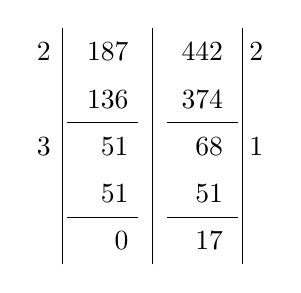
\begin{tikzpicture}[scale=.6]
\foreach \y/\ytext in {0/0,1/51,2/51,3/136,4/187}
{
    \node at (-1, \y)[left]{$\ytext$};
}    
\foreach \y/\ytext in {0/\boxed{17},1/51,2/68,3/374,4/442}
{
    \node at (1, \y)[left]{$\ytext$};
}   
\foreach \x in {-2.6,-.7,1.2}
{
    \draw (\x,-.5)--(\x,4.5);
}

\foreach \y in {.5, 2.5}
{
    \draw (-2.5,\y)--(-1,\y);
    \draw (-.4,\y)--(1.1,\y);
}
\node at (-3, 4) {2};
\node at (-3, 2) {3};
\node at (1.5, 4) {2};
\node at (1.5, 2) {1};
\end{tikzpicture}
\end{center}
$\therefore\quad (187,442)=17$



\begin{example}
求$(3887,2231)$.
\end{example}


\begin{solution}
\begin{center}
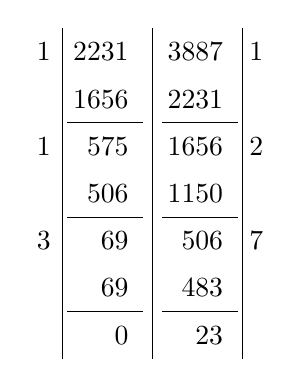
\begin{tikzpicture}[scale=.6]
\foreach \y/\ytext in {0/0,1/69,2/69,3/506,4/575, 5/1656, 6/2231}
{
    \node at (-1, \y)[left]{$\ytext$};
}    
\foreach \y/\ytext in {0/\boxed{23},1/483,2/506,3/1150,4/1656, 5/2231, 6/3887}
{
    \node at (1, \y)[left]{$\ytext$};
}   
\foreach \x in {-2.6,-.7,1.2}
{
    \draw (\x,-.5)--(\x,6.5);
}

\foreach \y in {.5, 2.5, 4.5}
{
    \draw (-2.5,\y)--(-.9,\y);
    \draw (-.5,\y)--(1.1,\y);
}
\node at (-3, 6) {1};
\node at (-3, 4) {1};
\node at (-3, 2) {3};
\node at (1.5, 6) {1};
\node at (1.5, 4) {2};
\node at (1.5, 2) {7};

\end{tikzpicture}

$\therefore\quad (3887,2231)=23$
\end{center}
\end{solution}



\begin{example}
求$(1547,3135)$.
\end{example}


\begin{solution}
\begin{center}
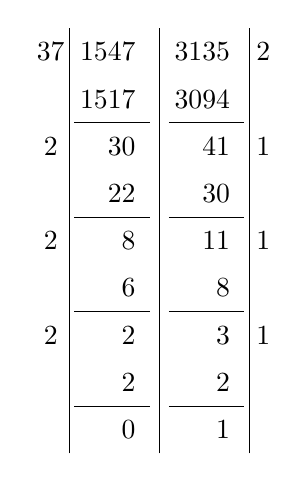
\begin{tikzpicture}[scale=.6]
\foreach \y/\ytext in {0/0,1/2,2/2,3/6,4/8, 5/22, 6/30, 7/1517, 8/1547}
{
    \node at (-1, \y)[left]{$\ytext$};
}    
\foreach \y/\ytext in {0/\boxed{1},1/2,2/3,3/8,4/11, 5/30, 6/41, 7/3094, 8/3135}
{
    \node at (1, \y)[left]{$\ytext$};
}   
\foreach \x in {-2.6,-.7,1.2}
{
    \draw (\x,-.5)--(\x,8.5);
}

\foreach \y in {.5, 2.5, 4.5, 6.5}
{
    \draw (-2.5,\y)--(-.9,\y);
    \draw (-.5,\y)--(1.1,\y);
}
\node at (-3, 8) {37};
\node at (-3, 6) {2};
\node at (-3, 4) {2};
\node at (-3, 2) {2};
\node at (1.5, 8) {2};
\node at (1.5, 6) {1};
\node at (1.5, 4) {1};
\node at (1.5, 2) {1};

\end{tikzpicture}

$\therefore\quad (1547,3135)=1\quad $ 可见,1547与3135是互质的.
\end{center}
\end{solution}

\begin{example}
  求$(435,783,928)$  
\end{example}

\begin{solution}
\begin{center}
    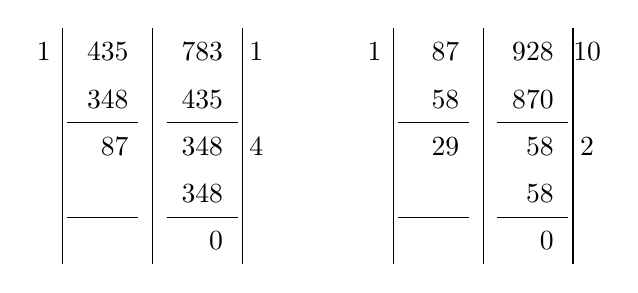
\begin{tikzpicture}[scale=.6]
    \begin{scope}
\foreach \y/\ytext in {0/{},1/{},2/\boxed{87},3/348,4/435}
{
    \node at (-1, \y)[left]{$\ytext$};
}    
\foreach \y/\ytext in {0/0,1/348,2/348,3/435,4/783}
{
    \node at (1, \y)[left]{$\ytext$};
}   
\foreach \x in {-2.6,-.7,1.2}
{
    \draw (\x,-.5)--(\x,4.5);
}

\foreach \y in {.5, 2.5}
{
    \draw (-2.5,\y)--(-1,\y);
    \draw (-.4,\y)--(1.1,\y);
}
\node at (-3, 4) {1};
\node at (1.5, 4) {1};
\node at (1.5, 2) {4};      
    \end{scope}


    \begin{scope}[xshift=7cm]
\foreach \y/\ytext in {0/{},1/{},2/\boxed{29},3/58,4/87}
{
    \node at (-1, \y)[left]{$\ytext$};
}    
\foreach \y/\ytext in {0/0,1/58,2/58,3/870,4/928}
{
    \node at (1, \y)[left]{$\ytext$};
}   
\foreach \x in {-2.6,-.7,1.2}
{
    \draw (\x,-.5)--(\x,4.5);
}

\foreach \y in {.5, 2.5}
{
    \draw (-2.5,\y)--(-1,\y);
    \draw (-.4,\y)--(1.1,\y);
}
\node at (-3, 4) {1};
\node at (1.5, 4) {10};
\node at (1.5, 2) {2};
    \end{scope}    
\end{tikzpicture}   

$\because\quad (435, 783) =87;\quad  (87,928)=29$

$\therefore\quad (435,783,928)=29$
\end{center}


\end{solution}

\begin{ex}
    用辗转相除法,求最大公约数:
\begin{multicols}{2}
\begin{enumerate}
    \item $(207,\; 1840)$ 
    \item $(429,\; 1848) $
    \item $(51425,\; 13310)$
    \item $(629,\; 259,\; 1073)$
    \item $(5688,\; 4977,\; 6636)$
\end{enumerate}

\end{multicols}
\end{ex}

\subsection{辗转相除法求最高公因式}
仿照前面求几个数的最大公约数的方法,同样地可以求几个一元多项式的最高公因式.只要把整数除法换成一元多项式除法即可.

设一元多项式$f(x)$与$g(x)$,如果$f(x)$的次数高于$g(x)$的次数.那么就用$g(x)$去除$f(x)$,得商$q_1(x)$,余$r_1(x)$.因而有:
\[f(x)=q_1(x)\cdot g(x)+r_1(x)\]
其中:$r_1(x)$的次数低于$g(x)$的次数,或为0.

所以,可得以下事实:
\begin{enumerate}
    \item 如果$r_1(x)=0$,那么$f(x)=q_1(x)\cdot g(x)$,这时必有:$(f(x),g(x))=g(x)$.如:
    
    由$x^3-1=(x^2+x+1)(x-1)$,$\therefore\quad (x^3-1,x-1)=x-1$.

\item 如果$r_1(x)\ne 0$,那么由$f(x)=q_1(x)\cdot g(x)+r_1(x)$与$r_1(x)=f(x)-q_1(x)\cdot g(x)$可以知道:
\[(f(x),g(x))=(g(x),r_1(x))\]

这就是说:求$(f(x),g(x))$的问题,可以换成求次数较低的多项式$g(x)$与$r_1(x)$的最高公因式问题.
\end{enumerate}


假如还嫌$g(x)$与$r_1(x)$的次数高,不易求得最高公因式,就可重复以上步骤,用$r_1(x)$去除$g(x)$,得到商式$q_2(x)$与余式$r_2(x)$,且有
\[g (x) =q_2 (x) \cdot r_1 (x) +r_2 (x) \]
其中,$r_2(x)$的次数又比$r_1(x)$的次数低,或等于0.

这时,若$r_2(x)=0$,则$(g(x),r_1(x))=r_1(x)$,从而$(f(x),g(x))=(g(x), r_1(x)) =r_1 (x)$.

若$r_2(x)\ne 0$,则与前边同理可有:
$$(r_1 (x), r_2(x))=(g(x),r_1(x))$$
从而就应有:
\[( f (x) ,g (x) ) = (g (x) ,r_1 (x))=(r_1(x),r_2(x))\]
这里$r_2(x)$的次数又比$g(x)$, $r_1(x)$的次数低了.

这样逐步地运用除法,就可以把所求两个多项式的最高公因式问题,转换成求两个次数较低的多项式的最高公因式问题.直到最后,自然就会求得$(f(x),g (x) )$.

这种方法,同样叫\textbf{辗转相除法}.



\begin{example}
如果$f(x)=x^4+x^3-2$, $g(x)=x^3-1$,试求$(f(x),g(x))$.
\end{example}


\begin{solution}
先求$f(x)$除以$g(x)$的商及余:
% \begin{center}
% \begin{tikzpicture}[yscale=.5]
% \foreach \y/\ytext in {0/x^4+x^3+0+0-2,-1/x^4+\,0+\,0-x\qquad,-2/x^3+0+x-2,-3/x^3+0+0-1,-4/x-1}    
% {
%     \node at (0,\y)[left] {$\ytext$};
% }
% \foreach \x in {.5,-1.5,-3.5}
% {
%     \draw (-3.5-\x*.2,\x)--(.5,\x);
% }



% \end{tikzpicture}
% \end{center}
\polylongdiv{x^4+x^3+0+0-2}{x^3+0+0-1}

$\therefore\quad f(x)=(x+1)\cdot g(x)+(x+1)$,并且
$(f(x),g(x))=(g(x), (x-1))$.

再求$g(x)$除以$x-1$的商及余.

\polylongdiv{x^3-1}{x-1}

$\therefore\quad g(x)=(x^2+x+1)(x-1)$,并且
$(g(x),x-1)=x-1$.

所以:$(f(x),g(x))=(g(x),(x-1))=x-1$,即:
$(f(x),g(x))=x-1$.

今后,在计算中,也不必象上面那样繁杂,可以采用以下分离系数的简便格式:
\begin{center}
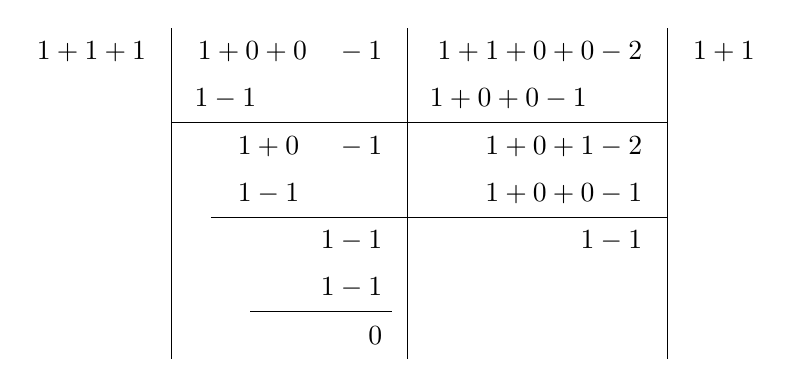
\begin{tikzpicture}[yscale=.6]
\foreach \y/\ytext in {6/1+0+0\quad -1  ,5/1-1\qquad\qquad \;\;  ,4/ 1+0\quad\; -1  , 3/ 1-1\qquad \quad , 2/1-1  , 1/1-1 ,0/ 0}
{
    \node at (-.2,\y)[left]{$\ytext$};
}

\foreach \y/\ytext in {6/1+1+0+0-2  ,5/1+0+0-1\qquad ,4/ 1+0+1-2  , 3/ 1+0+0-1  , 2/\boxed{1-1}}
{
    \node at (3.1,\y)[left]{$\ytext$};
}
\foreach \x in {-3,0,3.3}
{
    \draw(\x,6.5)--(\x, -.5);
}

\draw(-3,4.5)--(3.3,4.5);
\draw(-2.5,2.5)--(3.3,2.5);
\draw(-2,.5)--(-.2,.5);
\node at (-3.2,6)[left]{$1+1+1$};
\node at (3.5,6)[right]{$1+1$};
\end{tikzpicture}

\end{center}

$\therefore\quad (f(x),g(x))=x-1$

\end{solution}


\begin{example}
已知$\varphi(x)=\poly{1,0,3,0,3,0,1}$,$R(x)=\poly{1,0,3,1,2,1}$.

求:$(\varphi(x),R(x))$.
\end{example}


\begin{solution}
\begin{center}
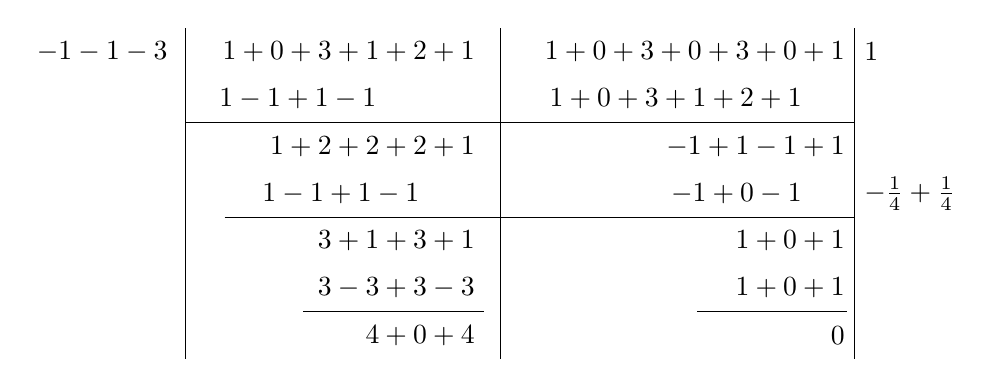
\begin{tikzpicture}[yscale=.6]
\foreach \y/\ytext in {6/1+0+3+1+2+1   ,5/1-1+1-1\qquad\quad\;\;   ,4/1+2+2+2+1  ,3/ 1-1+1-1\qquad   , 2/ 3+1+3+1 , 1/3-3+3-3, 0/4+0+4 }
{
    \node at (-.2,\y)[left]{$\ytext$};
}

\foreach \y/\ytext in {6/1+0+3+0+3+0+1  ,5/1+0+3+1+2+1\quad\;\;  ,4/ -1+1-1+1  , 3/ -1+0-1\quad\;\;   , 2/1+0+1, 1/1+0+1, 0/0}
{
    \node at (4.5,\y)[left]{$\ytext$};
}
\foreach \x in {-4,0,4.5}
{
    \draw(\x,6.5)--(\x, -.5);
}

\draw(-4,4.5)--(4.5,4.5);
\draw(-3.5,2.5)--(4.5,2.5);
\draw(-2.5,.5)--(-.2,.5);
\draw(2.5,.5)--(4.4,.5);
\node at (-4.1,6)[left]{$-1-1-3$};
\node at (4.5,3)[right]{$-\frac{1}{4}+\frac{1}{4}$};
\node at (4.5,6)[right]{$1$};
\end{tikzpicture}

\end{center}

$\therefore\quad (\varphi(x),R(x))=4x^2+4$,若不计零次因式,
则可得:
\[ (\varphi(x),R(x))=x^2+1 \]

\end{solution}

正由于最高公因式可以不计零次多项式的因式,所以,在辗转相除的过程中,为使运算简便,\textbf{可以将除式或被除式的各项同乘(或除)以一个非零数}.如例5.55可以这样做:
\begin{center}
\begin{tikzpicture}[yscale=.6]
\foreach \y/\ytext in {6/1+0+3+1+2+1   ,5/1-1+1-1\qquad\quad\;\;   ,4/1+2+2+2+1  ,3/ 1-1+1-1\qquad   , 2/ 3+1+3+1 , 1/3-3+3-3, 0/4+0+4, -1/\boxed{1+0+1} }
{
    \node at (-.2,\y)[left]{$\ytext$};
}

\foreach \y/\ytext in {6/1+0+3+0+3+0+1  ,5/1+0+3+1+2+1\qquad  ,4/ -1+1-1+1  , 3/ 1-1+1-1 , 2/1+0+1\qquad , 1/-1+0-1, 0/-1+0-1, -1/0}
{
    \node at (4.5,\y)[left]{$\ytext$};
}
\foreach \x in {-4,0,4.5}
{
    \draw(\x,6.5)--(\x, -1.5);
}

\draw(-4,4.5)--(4.5,4.5);
\draw(-3.5,2.5)--(-.2,2.5);
\draw(-2.5,.5)--(-.2,.5);
\draw(2.5,-.5)--(4.4,-.5);
\draw(2.2,1.5)--(4.4,1.5);
\node at (-4.1,6)[left]{$1+1+3$};
\node at (4.5,4)[right]{$1-1$};
\node at (4.5,6)[right]{$1$};

\node at (1,4) {(乘以$-1$)};
\node at (-3,0) {(除以4)};

\end{tikzpicture}

\end{center}

\[\therefore\quad  (\varphi(x),R(x))=x^2+1 \]

\begin{rmk}
 用分离系数写出辗转相除的格式时,一定要按未知数的降次标准形式将除式、被除式排好,缺项补上0.同时,要特别注意:辗转相除到能够整除时,前一步的余式,就是所求的最高公因式.   
\end{rmk}



\begin{example}
    求$f(x)=x^5+1$与$g(x)=x^3+3x^2+3x+1$的最高公因式.
\end{example}

\begin{solution}
\begin{center}
\begin{tikzpicture}[yscale=.6]
\foreach \y/\ytext in {6/1+3+3+1   ,5/2+6+6+2  ,4/2+3+1\qquad   ,3/ 3+5+2  , 1.5/ 3+\frac{9}{2}+\frac{3}{2} , 0/\frac{1}{2}+\frac{1}{2}, -1.5/\boxed{1+1} }
{
    \node at (-.2,\y)[left]{$\ytext$};
}

\foreach \y/\ytext in {6/1+0+0+0+0+1  ,5/1+3+3+1\qquad\quad\;\;   ,4/ -3-3-1+0+1  , 3/ -3-9-9-3\quad\;\;  , 2/6\;+8\;\;+3\;+1 , 1/6+18+18+6, 0/-10-15-5, -1/2\;+3\;+1, -2/2+2\quad\;\;\;\; , -3/1+1,  -4/1+1, -5/0 }
{
    \node at (3.8,\y)[left]{$\ytext$};
}

\foreach \x in {-3,0,4}
{
    \draw(\x,6.5)--(\x, -5.5);
}

\draw (-3,3.5)--(0,3.5);
\draw (-2,.75)--(0,.75);
\draw (0,4.5)--(4,4.5);
\draw (0,2.5)--(4,2.5);
\draw (0,.5)--(4,.5);
\draw (1,-2.5)--(4,-2.5);
\draw (2,-4.5)--(4,-4.5);


 \node at (-3.2,4)[left]{$1+\frac{3}{2}$};
 \node at (4.2,6)[right]{$1-3+6$};
 \node at (4.2,-1)[right]{$2+1$};

 \node at (4.2,0)[right] {(除以$-5$)};
 \node at (-3.2,0)[left] {(乘以2)};
 \node at (-3.2,6)[left] {(乘以2)};
\end{tikzpicture}

\end{center}

$\therefore\quad (f(x),g(x))=x+1$

\end{solution}


\begin{example}
求$(\poly{1,1,2,3}, \poly{1,1,1})$
\end{example}

\begin{solution}
同样用辗转相除法:
\begin{center}
\begin{tikzpicture}[yscale=.6]
\foreach \y/\ytext in {6/1+1+1   ,5/1+3\quad\;\;\;   ,4/-2+1  ,3/ -2-6  , 2/ 7 , 1/\boxed{1} }
{
    \node at (-.2,\y)[left]{$\ytext$};
}

\foreach \y/\ytext in {6/1+1+2+3  ,5/1+1+1\quad\;\;\;   ,4/ 1+3 , 3/ 1+3 , 2/0}
{
    \node at (2.8,\y)[left]{$\ytext$};
}

\foreach \x in {-2.5,0,3}
{
    \draw(\x,6.5)--(\x, 0.5);
}

\draw (-2.5,4.5)--(0,4.5);
\draw (0,4.5)--(3,4.5);
\draw (1,2.5)--(3,2.5);
\draw (-2.5,2.5)--(0,2.5);

\node at (-2.7,2)[left]{(乘以$\tfrac{1}{7}$)};
 \node at (-2.7,6)[left]{$1-{2}$};
 \node at (3.2,6)[right]{$1$};
 \node at (3.2,4)[right]{$1+3$};

\end{tikzpicture}

\end{center}

$\therefore\quad (\poly{1,1,1}, \poly{1,1,2,3})=1$
即:$\poly{1,1,1}$ 与 $\poly{1,1,2,3}$ 是互质的.

\end{solution}

如果要求两个以上多项式$f_1(x),f_2(x),f_3(x),\ldots$的最高公因式时,只要先求$(f_1(x),f_2(x))=d_1(x)$, 再求$(d_1(x),f_3(x))=d_2(x)$, 再求$(d_2(x), f_4 (x))=d_3(x),\ldots$, 这样依次求下去,即可求得:
\[(f_1 (x),\; f_2 (x),\; f_3 (x),\; f_4(x),\ldots)\]


\begin{example}
求$f_1(x)=x^4+x^3-x^2+x-2$,
$f_2 (x) =2x^4+5x^3-2x^2-7x+2$,$f_3(x)=\poly{3,-1,-1,0,-1}$,$f_4(x)=x^2-1$的最高公因式.
\end{example}

\begin{note}
在这里,除两两求最高公因式的方法外,也可以先求$(f_1(x),f_2(x))=d_1(x)$, 再求$(f_3(x), f_4(x))=d_2(x)$, 最后求$(d_1(x),d_2(x))=d(x)$,从而求得:
\[(f_1 (x) ,\; f_2 (x),\; f_3 (x),\; f_4 (x)) =d(x)\]
\end{note}

\begin{solution}
\begin{center}
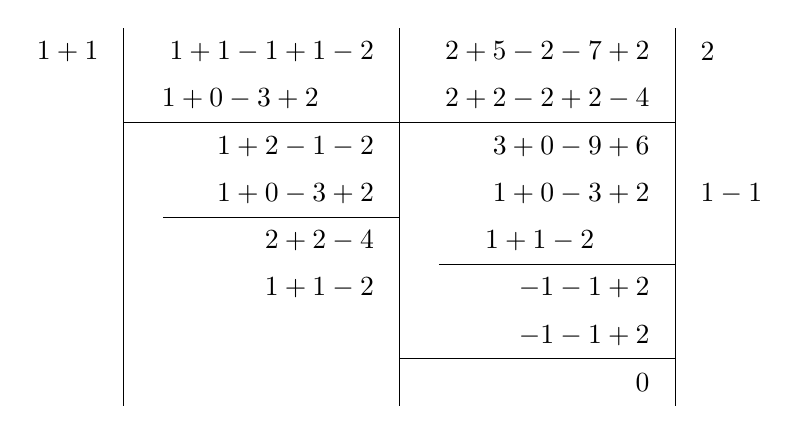
\begin{tikzpicture}[yscale=.6]
\foreach \y/\ytext in {6/1+1-1+1-2   ,5/1+0-3+2\qquad  ,4/1+2-1-2   ,3/ 1+0-3+2  , 2/2+2-4 ,1/\boxed{1+1-2} }
{
    \node at (.3,\y)[left]{$\ytext$};
}

\foreach \y/\ytext in {6/2+5-2-7+2  ,5/2+2-2+2-4  ,4/ 3+0-9+6 , 3/ 1+0-3+2  , 2/1+1-2\qquad  , 1/-1-1+2, 0/-1-1+2, -1/0}
{
    \node at (3.8,\y)[left]{$\ytext$};
}

\foreach \x in {-3,0.5,4}
{
    \draw(\x,6.5)--(\x, -1.5);
}

\draw (-3,4.5)--(4,4.5);

\draw (-2.5,2.5)--(.5,2.5);
\draw (.5,-.5)--(4,-.5);
\draw (1,1.5)--(4,1.5);

 \node at (4.2,6)[right]{$2$};
 \node at (4.2,3)[right]{$1-1$};
 \node at (-3.2,6)[left] {$1+1$};
\end{tikzpicture}

\end{center}

$\therefore\quad  (f_1(x), f_2 (x))=x^2+x-2=d_1(x)$

\begin{center}
\begin{tikzpicture}[yscale=.6]
\foreach \y/\ytext in {6/1+0-1   ,5/1-1\quad\;\;  ,4/1-1   ,3/ 1-1  , 2/0 }
{
    \node at (.3,\y)[left]{$\ytext$};
}

\foreach \y/\ytext in {6/3-1-1+0-1  ,5/3+0-3\qquad\;\; \quad ,4/ -1+2+0-1 , 3/ -1+0+1\qquad   , 2/2-1-1  , 1/2+0-2, 0/-1+1, -1/\boxed{1-1}}
{
    \node at (3.8,\y)[left]{$\ytext$};
}

\foreach \x in {-1.5,0.5,4}
{
    \draw(\x,6.5)--(\x, -1.5);
}

\draw (-1.5,4.5)--(4,4.5);

\draw (-1,2.5)--(.5,2.5);
\draw (1.5,.5)--(4,.5);
\draw (1,2.5)--(4,2.5);

 \node at (4.2,6)[right]{$3-1+2$};
 \node at (4.2,-1)[right]{(乘以$-1$)};
 \node at (-1.7,6)[left] {$-1-1$};
\end{tikzpicture}
\end{center}

$\therefore\quad (f_3(x),f_4(x))=x-1=d_2(x)$

显然,$(d_1(x),d_2(x))=(x^2+x-2,x-1)=x-1$,

$\therefore\quad (f_1(x),\; f_2(x),\; f_3(x),\; f_4(x))=x-1$

\end{solution}


\begin{ex}
用辗转相除法求最高公因式
\begin{enumerate}
    \item $f (x) =x^3-2x^2-2x-3,\qquad g (x) =2x^3+x^2+x-1$
    \item $g(x)=\poly{1,3,2,3,1},\qquad f(x)=\poly{2,5,-1,-1}$
    \item $f(x)=\poly{1,0,-2,9,-5,3},\qquad g(x)=\poly{1,-1,5,-3}$
    \item 求$(6x^4-6x^2,\; 3x^2-3,\; 8x^8-8x^4,\; 7x^7-7x^3)$
    \item $f(x)=\poly{1,-2,-4,4,-3}$,\qquad $g(x)=\poly{2,-5,-4,3}$,\qquad $\varphi(x)=x^2-9$
\end{enumerate}
\end{ex}




\subsection{公倍式与最低公倍式}
还是先从小学算术中所学的公倍数和最小公倍数复习开始:

如果一个整数$c$, 同时是数$a$和$b$的倍数,那么$c$就叫$a$、$b$的公倍数.而两个数的公倍数中,最小的一个正整数,叫做这两个数的\textbf{最小公倍数}.记作$[a,b]$.例如:4和6的公倍数有:$\pm 12,\pm 24,\pm 36,\ldots$, 但是,其中最小的一个正整数是12, 因此,$[4, 6]=12$.

在小学算术中,也学习了用分解质因数的方法求最小公倍数.

\begin{example}
求$[180, 240]$
\end{example}

\begin{solution}
\begin{center}
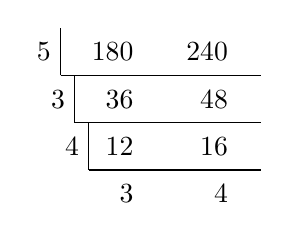
\begin{tikzpicture}[scale=.6]
\foreach \y/\ytext in {0/3, 1/12,2/36,3/180}
{
    \node at (0, \y)[left]{\ytext};
}
\foreach \y/\ytext in {0/4, 1/16,2/48,3/240}
{
    \node at (2, \y)[left]{\ytext};
}
\foreach \y/\x in {.5/4,1.5/3,2.5/5}
{
    \draw (-1-\y*0.3,\y)--(2.5,\y);
    \draw (-1-\y*.3,\y)--node[left]{\x}(-1-\y*.3,\y+1);
}

\end{tikzpicture}
\end{center}

$\therefore\quad [180, 240] =5\x3\x3\x4\x4=720$

这里我们也可知:$(180, 240)=5\x3\x4=60$.不难看出:
\[(180, 240)\cdot [180, 240]=180\x 240\]

\end{solution}

一般地,对任意两正整数$a,b$都有:
\[(a,b)\cdot [a,b]=a\cdot b  \]

由此,我们还可以用辗转相除先求出$(a,b)$, 进
而求出$[a,b]=\frac{a\x b}{(a,b)}$.


\begin{example}
求$[6731,\; 2809]$
\end{example}

\begin{solution}
\begin{center}
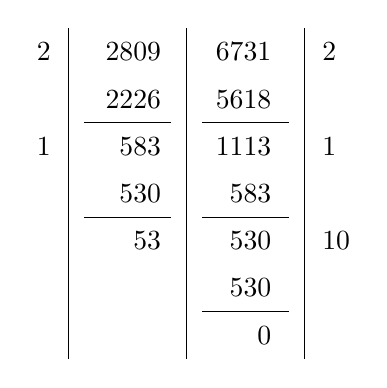
\begin{tikzpicture}[yscale=.6]
\foreach \x/\xtext in {6/2809, 5/2226, 4/583, 3/530, 2/\boxed{53}}
{
    \node at (-.2,\x)[left]{$\xtext$};
}

\foreach \x/\xtext in {6/6731, 5/5618, 4/1113, 3/583, 2/530, 1/530, 0/0}
{
    \node at (1.2,\x)[left]{$\xtext$};
}

\foreach \x in {0,-1.5,1.5}
{
    \draw (\x, -.5)--(\x, 6.5);
}

\draw (-1.3, 4.5)--(-0.2, 4.5);
\draw (0.2, 4.5)--(1.3,4.5);
\draw (-1.3, 2.5)--(-0.2, 2.5);
\draw (0.2, 2.5)--(1.3,2.5);
\draw (0.2, .5)--(1.3,.5);

\node at (-1.6,6)[left]{2};
\node at (-1.6,4)[left]{1};
\node at (1.6,6)[right]{2};
\node at (1.6,4)[right]{1};
\node at (1.6,2)[right]{10};

\end{tikzpicture}    
\end{center}

$\therefore\quad (6731,2809)=53$

因此,$[6731,\; 2809]=\frac{6731\x 2809}{53}=356743$

\end{solution}


\begin{example}
求$[513,\; 135,\; 3114]$.
\end{example}






\begin{solution}
\begin{center}
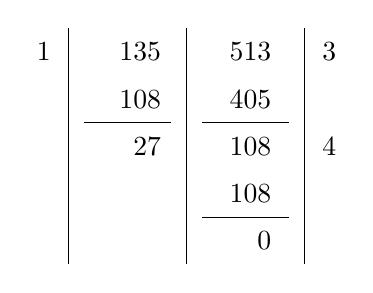
\begin{tikzpicture}[yscale=.6]
\foreach \x/\xtext in {6/135, 5/108, 4/\boxed{27}}
{
    \node at (-.2,\x)[left]{$\xtext$};
}

\foreach \x/\xtext in {6/513, 5/405, 4/108, 3/108, 2/0}
{
    \node at (1.2,\x)[left]{$\xtext$};
}

\foreach \x in {0,-1.5,1.5}
{
    \draw (\x, 1.5)--(\x, 6.5);
}

\draw (-1.3, 4.5)--(-0.2, 4.5);
\draw (0.2, 4.5)--(1.3,4.5);
\draw (0.2, 2.5)--(1.3,2.5);


\node at (-1.6,6)[left]{1};
\node at (1.6,6)[right]{3};
\node at (1.6,4)[right]{4};

\end{tikzpicture}    
\end{center}

$\therefore\quad (513,\; 135)=27$

$\therefore\quad [513,\; 135]=\frac{513\x 135}{27}=2565$

\begin{center}
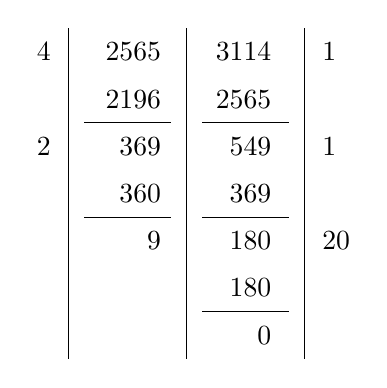
\begin{tikzpicture}[yscale=.6]
\foreach \x/\xtext in {6/2565, 5/2196, 4/369, 3/360, 2/\boxed{9}}
{
    \node at (-.2,\x)[left]{$\xtext$};
}

\foreach \x/\xtext in {6/3114, 5/2565, 4/549, 3/369, 2/180, 1/180, 0/0}
{
    \node at (1.2,\x)[left]{$\xtext$};
}

\foreach \x in {0,-1.5,1.5}
{
    \draw (\x, -.5)--(\x, 6.5);
}

\draw (-1.3, 4.5)--(-0.2, 4.5);
\draw (0.2, 4.5)--(1.3,4.5);
\draw (-1.3, 2.5)--(-0.2, 2.5);
\draw (0.2, 2.5)--(1.3,2.5);
\draw (0.2, .5)--(1.3,.5);

\node at (-1.6,6)[left]{4};
\node at (-1.6,4)[left]{2};
\node at (1.6,6)[right]{1};
\node at (1.6,4)[right]{1};
\node at (1.6,2)[right]{20};

\end{tikzpicture}    
\end{center}

$\therefore\quad (2565,\; 3114)=9$

$\therefore\quad [2565,\; 3114]=\frac{2565\x 3114}{9}=887490$

因而,$[513,\; 135,\; 3114]=887490$
\end{solution}

对于多项式,同样可以讨论它们的公倍式与最低公倍式.

如果多项式$\ell(x)$同时是多项式$f(x)$与$g(x)$的倍式,那么,$\ell(x)$就叫做它们的公倍式.而其中次数最低的公倍式,叫做\textbf{最低公倍式}.记作:$[f(x),g(x)]$.

例如:$x+1$与$x-1$的公倍式有:$x^2-1$, $2x^2-2$, $\frac{1}{3}x^2-\frac{1}{3}$, $x (x^2-1)$, $(x^2+1)(x^2-1),\ldots$.

通常所求多项式的最低公倍式,同样不考虑零次
式因式的差别.因而$x^2-1$, $2x^2-2$, $\frac{1}{3}x^2-\frac{1}{3}$看作
是一样的.它们之间只差一个非零常数倍.所以,
\[[x-1,\; x+1]=x^2-1\]

又如:$[3a^5b^2c,\; ab^4c^3d,\; 2a^2bc^6]=a^5b^4c^6d$.

就是说:最低公倍式等于各多项式中所有不同因式最高次方的连乘积.

\begin{example}
求$f(x)=6x^4-6x^2$与$g(x)=3x^2-3$的最低公倍式.
\end{example}

\begin{solution}
由于
\[\begin{split}
    f(x)&=6x^2(x^2-1)=6x^2(x+1)(x-1)\\
    g(x)&=3x^2-3=3(x+1)(x-1)
\end{split}\]
$\therefore\quad [f(x),\; g(x)]=x^2(x+1)(x-1)$
\end{solution}

显然,由于多项式的最高公因式与最低公倍式都不计零次因式,所以同样有:
\[[f (x) ,\; g (x) ] \cdot  (f (x) ,\; g (x) ) =k\cdot f (x) \cdot g (x) \]
其中,$k$是一个非零常数.

\begin{example}
求$\poly{1,3,2,3,1}$与$\poly{2,5,-1,-1}$的最低公倍式.
\end{example}

\begin{solution}
由辗转相除法可求得:
\[\left(\poly{1,3,2,3,1}, \; \poly{2,5,-1,-1}\right)=\poly{1,3,1}\]
因此:
\[\begin{split}
    &\quad \left[\poly{1,3,2,3,1}, \; \poly{2,5,-1,-1}\right]\\
    &=\frac{(\poly{1,3,2,3,1})\x (\poly{2,5,-1,-1})}{\poly{1,3,1}}\\
    &=(x^2+1)(\poly{2,5,-1,-1})
\end{split}\]

如果要求两个以上多项式的最低公倍式,和求最
小公倍数一样,可以两两逐步求出,只要每一步细心计算,是不难的.
\end{solution}




\begin{ex}
\begin{enumerate}
    \item 求下列各组数的最小公倍数:
    \begin{multicols}{2}
        \begin{enumerate}
        \item 96,\quad 84;
        \item 161,\quad 207;
        \item 1233,\quad 19180;
        \item 110,\quad 231,\quad 426;
        \item 236,\quad 354,\quad 767.
    \end{enumerate}
    \end{multicols}
    
    \item 求下列各组多项式的最低公倍式:
    \begin{enumerate}
        \item $2a^2b^3c,\quad 4b^2c^4d,\quad 6a^4d^2$
        \item $(x-1)^2(x+1),\quad 3(x-1)(x+1)^3,\quad 2 (x-1) (x+1)^2$
        \item $3x-1,\quad 9x^2-1,\quad 9x^2+1$
        \item $x^3-x^2+x-1,\quad x^3+x^2+x+1$
    \end{enumerate}
\end{enumerate}
\end{ex}

\section*{习题5.3}
\addcontentsline{toc}{subsection}{习题5.3}

\begin{enumerate}
\item 某校一年级一班有学生48人,二班有学生32人,两班共同组成几个宣传小队,要求组成的小队中每个班的同学人数相等、总人数也相等,而且所组成的小队数最少,问:能组成几队?每队几人?(求最大公约数)
\item 一排电杆,相邻两根间距都是45米.如果要改成间距60
米,且起点不动,那么从这根开始到第一根不动的电杆,距离是多少米?(求最小公倍数)
\item 小张、小王与小李三人做卫生值勤.小张8天轮一次,小王10天轮一次,小李12天轮一次.如果今天三人同时值勤,那么,至少几天后三人又能同时值勤?(求最小公倍数)
\item 求下列各组的最高公因式和最低公倍式:
\begin{enumerate}
    \item $9 x^{2} y z,\qquad -6 x y^{2} z,\qquad 24 x y^{2}$
    \item $-3(a-b)^{3},\qquad -6(a-b)\left(a^{2}+a b+b^{2}\right),\qquad -8(a-b)^{2}(a+b)$
    \item $x^{2}-y^{2},\qquad  x^{4}-y^{4}$
    \item $m^{2}-4 n^{2},\qquad  m^{2}+m n-2 n^{2},\qquad m^{2}+3 m n+2 n^{2}$
\end{enumerate}

\item 求下列各组多项式的最高公因式和最低公倍式:
\begin{enumerate}
    \item $x^{2}-3 x y+2 y^{2},\qquad  x^{2}+2 x y-8 y^{2}$
    \item  $m^{2}-m-6,\qquad  m^{2}-2 m-3 $
    \item $y^{4}-9 y^{2},\qquad  y^{3}-5 y^{2}+6 y$
    \item  $24 a^{4} b-24 a^{3} b^{2}+6 a^{2} b^{3}, \qquad  36 a^{3} b^{2}-36 a^{2} b^{3}+9 a b^{4}$
    \item ${a}^{3}-3 a^{2}+2 a,\qquad  a^{4}-a^{2},\qquad  a^{2}+a-2$
    \item  $x^{2}-x-2,\qquad  x^{2}+14 x-32,\qquad  x^{2}-5 x+6$
    \item  $8 x^{3}-27,\qquad 24 x-8 x^{2}-18,\qquad 27-54 x+36 x^{2}-8 x^{3}$ 
    \item  $-6 x y\left(x^{2}-3 x y+2 y^{2}\right),\qquad  4 x^{3} y^{2}\left(x^{2}-x y-2 y^{2}\right)$
\end{enumerate}

\item 求最高公因式与最低公倍式.
\begin{enumerate}
\item $\left(b^{2}-2 b\right)^{4},\qquad   \frac{1}{8}\left(b^{2}-2 b\right)^{2},\qquad  \left(b^{2}-2 b\right)^{3} ;$
\item $6\left(4 x^{2}-1\right),\qquad   4-8 x ,\qquad   12\left(4 x^{2}-4 x + 1\right)$
\item $12\left(x^{4}-y^{4}\right),\qquad   10\left(x^{6}-y^{6}\right),\qquad   8\left(x^{4} y+x y^{4}\right)$
\item $x^{2}-x, \qquad  2 x^{2}-6 x,\qquad   x^{3}-x$
\item $(x-1)(x-2),\qquad   5 x^{4}-15 x^{3}+8 x^{2}+6 x-4$
\item $x^{3}-1,\qquad   x^{3}-4 x^{2}-4 x-5$
\item $(x-1)^{2}(x-2)^{2},\qquad (\poly{1,-3,2})(\poly{2,-5,5,-6})$
\item $(x^2-1)^2(x+1)^2,\qquad (\poly{1,5,7,3})(\poly{1,-6,-7})$
\end{enumerate}

\item 用辗转相除法求最高公因式$(f(x),g(x))$.
\begin{enumerate}
    \item $f(x)=\poly{1,1,2,2},\qquad g(x)=\poly{1,2,3,2}$
    \item $g(x)=\poly{2,-1,-1,1},\qquad f(x)=\poly{1,-1,1,-2}$
    \item $f(x)=\poly{2,3,4,2,1},\qquad g(x)=\poly{2,-1,2,0,1}$
    \item $g(x)=\poly{1,1,-1,1,-2},\qquad f(x)=\poly{2,5,-2,-7,2}$
    \item $f(x)=\poly{1,-2,1,-1,2,-1},\qquad g(x)=\poly{5,-8,3,-2,2}$
\end{enumerate}

\item 求最低公倍式$[f(x),g(x)]$
\begin{enumerate}
    \item $g(x)=\poly{6,1,-44,21},\qquad f(x)=\poly{3,-13,23,-21}$
    \item $f(x)=\poly{6,-3,7,1,-3},\qquad g(x)=\poly{2,3,7,3,9}$
    \item $g(x)=\poly{1,0,0,0,1},\qquad f(x)=\poly{1,0,0,-1}$
\end{enumerate}

\end{enumerate}

\section*{本章内容要点}

这一章是第四章多项式理论的继续和深入,主要内容有:因式分解、余式定理及其推论和应用、辗转相除法及其应用.

一、在指定范围内,把一个多项式写成几个次数
较低的不可约多项式之积的变形,就是多项式的因式分解.

多项式因式分解的常见方法有:
\begin{enumerate}
    \item 提取公因式法;
    \item 分组分解法;
    \item 乘法公式分解法;
    \item 配方法、视察法分解二次三项式;
    \item 待定系数法分解二元二次多项式.
\end{enumerate} 

二、余式定理是:多项式$f(x)$除以$(x-a)$所得
的余式是$f(a)$,即
\[f (x) =q (x) \cdot (x-a) +f (a) \]
由此,可以得到以下推论:
\begin{enumerate}
\item 如果$f(a)=0$(或说$a$为$f(x)$的根),那么,$f(x)$
可以被$(x-a)$整除.反过来也正确.
\item 如果$f(a)=0,f(b)=0$(或说$a,b$为$f(x)$的两个不同的根),那么,$f(x)$必可以被$(x-a)(x-b)$整除,也就是$f(x)$必含有因式$(x-a)(x-b)$.反过来说,也是正确的.
\item 一元$n$次多项式$f(x)$,至多只能有$n$个不同的根.
\item  如果:已知$f(a_1),f(a_2),f(a_3),\ldots,f(a_{n+1})$
共$n+1$个值,那么,就可以确定一个$n$次多项式.
\end{enumerate}

三、综合运用余式定理及其推论、综合除法及待
定系数法,可以进行因式分解、求整系数多项式的有理根.

在这里,可以进一步发现,解方程与因式分解是互通的.因为:
如果$f(x)$可以分解为$(mx+n)\cdot (px+q)\cdots (rx+s)$,那么,方程$f(x)=0$就一定有有理根$-\frac{n}{m},-\frac{q}{p},\ldots,-\frac{s}{r}$.

反过来,如果方程$f(x)=0$有有理根$-\frac{b}{a},-\frac{d}{c},\ldots,-\frac{f}{e}$.那么,多项式$f(x)$就一定含有因式:$(ax+b)(cx+d)\cdots(ex+f)$.

四、辗转相除法

利用辗转相除法,可以求出几个多项式的最高公因式和最低公倍式.

两个多项式$f(x)$与$g(x)$的最高公因式记为:$(f(x),g(x))$;最低公倍式记为:$[f(x), g(x)]$.由于它们都不计非零常数因子,因而有以下关系式:
\[ kf (x) g (x) = (f(x), g(x))\cdot [f(x),g(x)]\]
\[[f(x),g(x)]=\frac{f(x)\cdot g(x)}{(f(x), g(x))}\qquad \text{(非零常数$k$不计)}\]



\section*{复习题五}
\addcontentsline{toc}{section}{复习题五}

\begin{enumerate}
\item 分解因式:
\begin{multicols}{2}
    \begin{enumerate}
    \item $\left(x^{2}+3 x\right)^{2}-(2 x+6)^{2}$
    \item $2 a^{3}-7 a^{2} b+3 a b^{2} ;$
    \item  $x^{3}+x^{2} y-x y^{2}-y^{3}$
    \item  $x^{6}-3 x^{4}+2 x^{2}$
    \item  $\left(a^{2}-b^{2}+1\right)^{2}-4 a^{2} b^{2}$
    \item  $a^{4}-5 a^{2} b^{2}+4 b^{4}$
    \item  $x^{8}-y^{8}$
    \item  $x^{9}+y^{9}$
    \item  $15 x^{2 n+3}-25 x^{n+1}$ 
    \item  $(a+b)^{3}+125$
    \item  $a^{2}+b^{2}+x^{2}-y^{2}-2(a x-b y)$
    \item  $\left(a^{2}+a\right)^{2}-10\left(a^{2}+a\right)+25$
    \item  $a^{2} b^{2}+a b+\frac{1}{2} c-\frac{1}{4} c^{2}$ 
    \item  $4 x^{2} y^{4}+2 x y^{2}-9 z^{2}-3 z$
    \item  $(a-b)^{3}-4(a-b)^{2}+4(a-b)$
    \item  $0.7 m^{3}+1.4 m^{2}+0.7 m n^{2}$ 
    \item  $x y+x^{2}+\frac{1}{4} y^{2}$
    \item  $9 x^{2}-4 y^{2}-z^{2}+4 y z$
\end{enumerate}
\end{multicols}

\item 分解因式:
\begin{multicols}{2}
\begin{enumerate}
    \item $4 x^{4}+y^{4} $
    \item $a^{4}-23 a^{2}+1$
    \item $x^{4}-x^{2}+8 x-16$
    \item $x^{4}-2 x^{3}+x^{2}-16$
    \item $(a x+b y)^{2}+(b x-a y)^{2}$
    \item   $x y z-y z-z x-x y+x+y+z-1$
    \item  $x^{2}+y^{2}+z^{2}+2 y z+2 x z+2 x y$
    \item  $a^{2}+b^{2}+c^{2}-2 a b+2 a c-2 b c$
\end{enumerate}
\end{multicols}

\item 先化简, 再将结果分解因式.
\begin{enumerate}
    \item  $x(4 x-5)+(1+3 x)(1-3 x)-3(x-2)(x+3)-3$
\item  $\left(2 x^{2}+3 x-1\right)\left(2 x^{2}-3 x+2\right)+(4 x-1)(x-2)-1$
\end{enumerate}

\item 先将被除式分解因式, 再求商.
\begin{enumerate}
    \item $\left[(a+b)^{3}-c^{3}\right]\div (a+b-c)$
    \item $\left(a^{3}+6 a^{2} b+12 a b^{2}+8 b^{3}\right)\div (a+2 b)$
\end{enumerate}

\item 分解因式:
\begin{multicols}{2}
\begin{enumerate}
    \item $x^{3}+x^{2}+x+1$
\item $x^{4}-2 x^{2}-8 x+5$ 
\item $3 x^{3}+2 x^{2} y-19 x {y}^{2}+6 y^{3}$
\item $6 x^{3}-13 x^{2} y-14 x y^{2}-3 y^{3}$
\end{enumerate}
\end{multicols}
\item 用待定系数法分解因式:
\begin{enumerate}
\item $2 x^{2}-5 x y-3 y^{2}+x+11 y-6$
\item $x^{2}-5 x y+6 y^{2}-x+y-2 $
\item $x^{2}+3 x y+2 y^{2}+3 z x+5 y^{3}+2 z^{2}$
\end{enumerate}


\item 如果$f(x)$除以$(x-1)$的余数为2,试求:$x^2\cdot f(x)-3f(x)$除以$(x-1)$所得的余数.

\item 试证明:$f(x)=2x^2+7x+9$除以$ax+b$ 的余式总是正数.
\item 
\begin{enumerate}
\item 已知多项式$f(x)=x^4-3x^3+6x^2+ax+b$含有因式$x^2-1$,试求:$a$、$b$的值.
\item 已知$f(x)=ax^4+bx^3+1$能被$(x-1)^2$整除,试求$a$与$b$的值.
\end{enumerate}

\item 
\begin{enumerate}
\item 如果 $b_n+b_{n-1}+\cdots+b_1+b_0=0$,试证明:多项式$f(x)=b_nx^n+b_{n-1}x^{n-1}+\cdots+b_1x+b_0$必有一个因式$x-1$;
\item 证明:$(x+1)^{2n}-x^{2n}-2x-1$能被$(x+1)\cdot (2x+1)$整除.
\end{enumerate}

\item 证明以下各题:
\begin{enumerate}
    \item 若$n$为偶数,$n^3-n$可被6整除;若$n$为奇数,$n^3-n$可被24整除;
    \item $53^{53}-33^{33}$可被10整除;
    \item 四个连续自然数的乘积加1,必是一个完全平方数;
    \item 若一数除以5余1,另一数除以5余2,则这两个数的平方和能被5整除.
\end{enumerate}

\item 已知方程$(m+1)(x^2-x)=(m-1)(x-1)$有两个互为相反数的根,试用韦达定理求出$m$的值.
\item 已知方程$x^3-6x^2+kx-6=0$的三个根为:$a-d,a,a+d$试求它的三个根及$k$值.
\item 求作一个方程,使它的三个根分别为方程 $x^3-2x^2-x+2=0$的三个根的倒数.

\item 求最高公因式及最低公倍式.
\begin{enumerate}
    \item $g(x)=\poly{1,1,-1,0,-2,-1},\qquad f(x)=\poly{3,2,0,2,-3}$
    \item $g(x)=\poly{3,-5,4,-2,1},\qquad f(x)=\poly{3,-2,1,-1}$
    \item $g(x)=\poly{1,2,3,2,0},\qquad f(x)=\poly{1,1,2,2,0}$
\end{enumerate}


\item 如果$ax^2+bx+c$与$cx^2+bx+a$的最高公因式是$x$的一次多项式,试证明:
$a+b+c=0$或$a-b+c=0$.
\item 两个用相同字码组成的二位数(都是质数)的差是一个完全平方数.试求这两个数.
\item 若$a,b,\sqrt{a^2-4b}$都是自然数,证明:方程$x^2-ax+b=0$的根也是自然数.

\end{enumerate}

